\documentclass[a4paper, 12pt]{article}
\usepackage[fontsize=12pt]{scrextend}

% ABNT - PACOTE DE ACENTUAÇÃO
\usepackage[utf8]{inputenc} 

% MARGENS LEFT RIGHT TOP E BOTTOM
\usepackage[lmargin=2cm,
            tmargin=0.6cm,
            rmargin=2cm,
            bmargin=3cm,
            headsep=0.0cm,
            includeheadfoot]{geometry}

\setlength\headheight{2.8cm}

% LEVA O ESTILO DO TEXTO PARA OUTROS PROGRAMAS TIPO WORD
\usepackage[T1]{fontenc}

% PÕE O PRIMEIRO PARÁGRAFO AUTOMATICAMENTE
\usepackage{indentfirst}

% HABILITA A UTILIZAÇÃO DE FONTES
\renewcommand{\familydefault}{\sfdefault}

\usepackage[onehalfspacing]{setspace}  % ESPAÇAMENTO ENTRE AS LINHAS
\usepackage[brazil]{babel}             % TRADUZ PARA PORTUGUÊS
\usepackage{comment}                   % COLOCAR COMENTÁRIOS
\usepackage{enumerate}                 % PACOTE PARA ENUMERAÇÃO
\usepackage{multirow, multicol}        % FORMATAR TABELAS
\usepackage{colortbl}                  % TABULAR COM COR 
\usepackage{lipsum}                    % TEXTO ALEATORIO
\usepackage{dashrule}                  % USAR LINHAS PONTILHADAS
\usepackage{paracol}                   % TEXTOS EM COLUNAS
\usepackage{hyperref}                  % HIPERLINKS NO SUMÁRIO

\pagestyle{empty}       % PREENCHIMENTO DA PÁGINA (FANCY HABILITA)
\usepackage{fancyhdr}   % CABEÇALHO E RODAPÉ
\fancyhf{}              % SEM NUMERAÇÃO NO MEIO PÁGINA

\usepackage{graphicx}   % PACOTE PARA IMAGENS
\usepackage{efbox}      % PACOTE PARA BORDAS EM IMAGENS
\usepackage{subfig}     % IMAGENS LADO A LADO
\usepackage{float}      % POSICIONAR IMAGEM NO COMANDO FIGURE
\usepackage{tabularx}   % PARA TABULAR MAIS BONITO

% HABILITAR CORES PARA TEXTOS E CAIXAS DE TEXTO COLORIDAS
\usepackage[x11names]{xcolor}

% COR TOPICOS \SECTION{}
\usepackage{sectsty}

% CAIXA DE TEXTO COLORIDA COM TÍTULO
\usepackage{wrapfig}
\usepackage[most]{tcolorbox}

% MATEMÁTICA
\usepackage{mathrsfs}
\usepackage{amsmath}
\usepackage{amsthm}
\usepackage{amsfonts}
\usepackage{amssymb}
\usepackage{dsfont}
\usepackage{mathtools}
\usepackage{tikz}                        
\usetikzlibrary{babel,quotes, angles}   % ÂNGULOS
\usepackage{esvect}                     % VETORES \vv{}
\everymath{\displaystyle}               % FRAÇÕES MAIS BONITAS

% \cancel{x}, \bcancel{x} (invertido), \cancelto{x}{para y}   
\usepackage{cancel}

% OUTROS
%\usepackage{parskip}        % ALINHAMENTO TEXTO (ELIMINA PARÁGRAFOS)
\usepackage{blindtext}      % IMPRIME TEXTO ALEATÓRIO \blindtext
\usepackage{fancybox}       % MARGENS CUSTOMIZÁVEIS

% FONTE MATEMÁTICA
\DeclareMathVersion{testemath}
\SetSymbolFont{operators}{testemath}{OT1}{bch}{n}{n}
\SetSymbolFont{letters}{testemath}{OML}{bch}{n}{n}
\mathversion{testemath}     % IMPORTANDO OS PACOTES
% NOVOS COMANDOS PARA TÓPICOS E CORES
\newcommand{\espaco}{\hspace{0.2cm}}
\newcommand{\espacolongo}{\hspace{1cm}}
\newcommand{\derivada}{\frac{d}{dx}}
\newcommand{\seta}{$\rightarrow\,\,\,$}
\newcommand{\Seta}{$\Rightarrow\,\,\,$}
\newcommand{\obs}{\color{red} Obs: \color{black}}
\newcommand{\linha}{\noindent\rule{20cm}{0.4pt}}
\newcommand{\ponto}{\textbullet \hspace{0.1cm}}
\newcommand{\cor}[2]{\color{#1}#2\color{black}}
\newcommand{\cors}[2]{\color{#1}#2 \color{black}}
\newcommand{\quadrado}{\scalebox{0.8}{$\,\, \blacksquare \,\,$ }}

% COMANDOS PARA CAIXAS COLORIDAS E TEXTOS ESTÉTICOS
\newcommand{\blueText}[1]{
    \color{DeepSkyBlue2} #1 \color{black}
}
\newcommand{\ex}[1]{
    \colorbox{DeepSkyBlue2}{\color{white}\textbf{EXEMPLO #1}\color{black}}
}
\newcommand{\legenda}[1]{
    \colorbox{DeepSkyBlue2}{\color{white}\textbf{#1}\color{black}}
}
\newcommand{\legendaMatematica}[2]{
    \phantom{#2} \hfill $#1$ \hfill #2
}
\newcommand{\centermat}[1]{
    \begin{center} $#1$ \end{center}
}
\newcommand{\cvsection}[2][]{
  \bigskip \bigskip{\color{black} \LARGE \bfseries \MakeUppercase{#2}}\\[-1ex]
  \color{orange}\rule{\linewidth}{2pt} \\ \color{black}
}
\newcommand{\cvtag}[1]{
  \tikz[baseline]\node[anchor=base,draw=black!80!white,rounded corners,inner xsep=1ex,inner ysep=0.75ex,text height=1.5ex,text depth=.25ex]{\color{gray}#1\color{black}};
  \vspace{0.25ex}
}
\newcommand{\cvlang}[2]{%
    \textcolor{black}{\textbf{#1:}}
    \textcolor{blue!70!black}{\textbf{#2}}
}
\newcommand{\divider}{
    \textcolor{black!80!white!30}{\hdashrule{\linewidth}{0.6pt}{0.5ex}}\smallskip
}
\newcommand{\topico}[1]{
    \large\color{red}#1\normalsize \color{black} \\
}
\newcommand{\titulo}[1]{
    \begin{center} \Large \color{blue} #1 \normalsize \color{black} \end{center}
}
\newcommand{\fillPage}[1]{
    \color{white} a \color{black}
    \vfill  
    
    #1
    
    \vfill
    \color{white} a \color{black}
    \newpage
}
\newcommand{\modeloTeorema}[2]{
    \begin{center}
    \begin{minipage}{.8\linewidth}
        \tcbset{
            enhanced,            % ESTILO DO QUADRO
            left=5mm,            % ESPAÇAMENTO ESQUERDO
            right=5mm,           % ESPAÇAMENTO DIREITO
            top=5mm,             % ESPAÇAMENTO SUPERIOR TEXTO
            bottom=5mm,          % ESPAÇAMENTO INFERIOR TEXTO
            boxrule=1pt,         % GROSSURA DAS LINHAS DE BORDA
            fonttitle=\bfseries, % ESTILO DA FONTE DO TÍTULO
            toptitle=2mm,   % ESPAÇAMENTO SUPERIOR TITULO
            bottomtitle=2mm % ESPAÇAMENTO INFERIOR TITULO
        }
        \begin{tcolorbox}[
            colback=blue!25!white,     % COR DO FUNDO DO TEXTO
            colframe=orange!70!yellow, % COR DO FUNDO DO TÍTULO
            title=\centering \color{black} #1
            ]
            #2
        \end{tcolorbox}
    \end{minipage}
    \end{center}
}
\newcommand{\titleBox}[4]{
    \begin{center}
    \begin{minipage}{.#1\linewidth}
        \tcbset{
            enhanced, left=4mm, right=4mm,top=4mm,
            bottom=4mm,boxrule=2pt
        }
        \begin{tcolorbox}[colback=#2]
            \color{#3} \Large \bfseries \centering
            #4
        \end{tcolorbox}
    \end{minipage}
    \end{center}
}
\newcommand{\bigpar}[1]{
    \bigg( #1\bigg )
}
\newcommand{\bordaImagem}[2]{
    \efboxsetup{linecolor=black,linewidth=#1, margin=0pt}
    \efbox{#2}
}

\newcommand{\referencia}[5]{
    \begin{flushleft} \noindent \justify \small
        \hypertarget{#1}{}
        #1. #2, #3. Disponível em: #4. Acesso em: #5.
    \end{flushleft}\vspace{-1cm}
}        % IMPORTANDO AS FUNÇÕES
\usepackage{helvet}  % USANDO A FONTE ARIAL
\usepackage{minted}
\usepackage{ragged2e}
\usepackage{longtable}
\usepackage{url}
\usepackage{xurl}
\usepackage{adjustbox}  % no preâmbulo


\newcommand{\fcol}[2]{
    \multicolumn{1}{|m{#1 cm}|}{\centering #2} 
}

\newcommand{\col}[2]{
    \multicolumn{1}{m{#1 cm}|}{\centering #2} 
}


\makeatletter
\renewcommand\tableofcontents{%
    \centering
    \section*{\contentsname
        \@mkboth{%
           \MakeUppercase\contentsname}{\MakeUppercase\contentsname}}%
    \@starttoc{toc}%
    }
\makeatother


% INICIANDO DOCUMENTO
\begin{document}
\fancypagestyle{modeloTexto}{
    % MOSTRA CABEÇALHO E NÚMERO DE PÁGINAS
    \pagestyle{fancy}
    
    \chead{
        \begin{center}
            
\includegraphics[width=17cm]{imagensCapa/head.png}
        \end{center}
    }
    
    % CABEÇALHO NO CANTO INFERIOR ESQUERDO
    \lfoot{}
    
    % CABEÇALHO NO CANTO INFERIOR DIREITO
    \rfoot{}

    \cfoot{
        \vspace{-0.7cm}
        \thepage
    }
    
    % ESPESSURA DA LINHA DO CABEÇALHO (0 ELIMINA ESSA LINHA)
    \renewcommand{\headrulewidth}{0pt}    
}

\fancypagestyle{modeloReferencias}{
    % MOSTRA CABEÇALHO E NÚMERO DE PÁGINAS
    \pagestyle{fancy}
    
    % CABEÇALHO NO CANTO SUPERIOR ESQUERDO
    \lhead{}
        
    % CABEÇALHO NO CANTO SUPERIOR DIREITO -> \RIGHTMARK MOSTRA A SUBSECTION
    \rhead{}
    
    % CABEÇALHO NO CANTO INFERIOR ESQUERDO
    \lfoot{}
    
    % CABEÇALHO NO CANTO INFERIOR DIREITO
    \rfoot{}
    
    % ESPESSURA DA LINHA DO CABEÇALHO (0 ELIMINA ESSA LINHA)
    \renewcommand{\headrulewidth}{0pt}   
}

\pagestyle{modeloTexto}
\begin{center}
    \LARGE
    \textbf{RELATÓRIO DE MACROENTREGA 2}

    \vspace{0.6cm}
    \normalsize

    \begin{minipage}{.90\linewidth}
        \centering
        \textbf{
            Dispositivo Referência de Monitoramento dos Movimentos em Helidecks e Guindastes Offshore
        }
    
        \vspace{.6cm}
        \textbf{PIFF-2411.0049}
        \normalsize
    \end{minipage}
    
    \vspace{1.2cm}
    
    \begin{flushleft}
     \phantom{a.}\textbf{Período: 05/03/2025 a 04/07/2025}
    \end{flushleft}
    
    \begin{center}
    \small
    \begin{tabular}{|c|c|c|}
    \hline
        Item & Produto & Critérios de Aceitação \\
    \hline
        \multicolumn{1}{|m{5cm}|}{
            4.1 Componentes Eletrônicos
        } 
        & \multicolumn{1}{m{3.5cm}|}{
            \centering
            Relatório
        } 
        & \multicolumn{1}{m{6.5cm}|}{
            Relatório contendo informações referentes aos componentes eletrônicos pesquisados e adquiridos para o projeto.
        }\\
    \hline
        \multicolumn{1}{|m{5cm}|}{
            4.2 Componentes Eletrônicos
        } 
        & \multicolumn{1}{m{3.5cm}|}{
            \centering
            Relatório
        } 
        & \multicolumn{1}{m{6.5cm}|}{
            Relatório contendo
            informações referentes a
            todo material de consumo
            pesquisado e adquirido
        }\\
    \hline
        \multicolumn{1}{|m{5cm}|}{
            5.1 Projeto das Placas de Circuitos impressos
        } 
        & \multicolumn{1}{m{3.5cm}|}{
            \centering
            Esquemático
        } 
        & \multicolumn{1}{m{6.5cm}|}{
            Aprestar o esquemático,
            testes funcionais do circuito
        }\\
    \hline
        \multicolumn{1}{|m{5cm}|}{
            5.2 Projeto do Circuito Eletrônicos/sensores
        } 
        & \multicolumn{1}{m{3.5cm}|}{
            \centering
            Esquemático
        } 
        & \multicolumn{1}{m{6.5cm}|}{
            Apresentar o esquemático e
            testes funcionais do circuito
        }\\
    \hline
        \multicolumn{1}{|m{5cm}|}{
            5.3 Projeto de Design da Embalagem
        } 
        & \multicolumn{1}{m{3.5cm}|}{
            \centering
            Desenho Técnico
        } 
        & \multicolumn{1}{m{6.5cm}|}{
            Apresentar os estudos para
            melhor
            especificação do que será
            instalado nas estruturas
            Offshore.
        }\\
    \hline
    \end{tabular}
\end{center}

    \vfill
    \centering
    Polo de Inovação\\
    Campos dos Goytacazes\\
    2025

    \newpage

    \vfill
    \textbf{DIRETOR DO PICG}\\
    Vicente de Paulo Santos de Oliveira
    \vfill
    
    \textbf{DIRETOR DE INOVAÇÃO TECNOLÓGICA}\\
    Rogério Atem de Carvalho
    \vfill
    
    \textbf{DIRETORA DE GESTÃO DE PROJETOS}\\
    Juliana Gonçalves Vidigal
    \vfill
    
    \textbf{COORDENADOR DO PROJETO}\\
    Robson da Cunha Santos
    \vfill
    
    \textbf{PESQUISADORES}\\
    Gerson Gomes Cunha\\
    Milena Bissonho Soares\\
    Letícia Barcelos Reis \\
    Matheus Ribeiro Vidal
    \vfill
    
    \textbf{ESTUDANTES}\\
    Jean Viana Ribeiro \\
    Klauss Miranda Marchi \\
    Matteus Araujo Ouverney\\
    Danilo Ricardo Lima de Oliveira
    \vfill

    \textbf{VOLUNTÁRIOS}\\
    Gabriel Renato Pereira Campos\\
    Levy da Silva Monteiro\\
    Pedro Freitas Machado\\
    Lucas Marvilla Andrade Pinheiro
    \vfill
\end{center}

\newpage
\tableofcontents
\newpage
\listoffigures
\newpage
\listoftables
\newpage
\raggedright
\justifying
\normalsize


\newpage
\section{Introdução}
    O presente relatório corresponde à Macroentrega II do projeto “Dispositivo Referência de Monitoramento dos Movimentos em Helidecks e Guindastes Offshore” (PIFF-2411.0049). Esta fase do projeto tem como foco central o desenvolvimento do hardware embarcado, cobrindo desde a pesquisa e aquisição dos componentes eletrônicos e materiais de consumo até a definição dos esquemáticos das placas de circuito impresso e o projeto de design da embalagem para instalação em ambiente offshore.

    Paralelamente ao escopo inicial, foram elaborados novos protótipos baseados em microcontroladores de baixa complexidade e desenvolvidos algoritmos de fusão sensorial e filtros avançados, com o objetivo de documentar os progressos nesses domínios. Para isso, constituiu-se uma equipe especializada, responsável pela criação de códigos proprietários de alto desempenho, fundamentais aos próximos estágios de desenvolvimento, visando assegurar um sistema embarcado competitivo e de custos adequados.
    
    Outrossim, a elaboração dos primeiros esquemas dos protótipos, assim como o desenvolvimento da embalagem, foi conduzida por duas equipes distintas, cujos resultados encontram-se anexados neste documento. Após a finalização de todos os componentes, será confeccionada uma PCB (placa de circuito impresso) para a realização dos testes do protótipo geral do projeto. Esses ensaios terão como objetivo verificar o desempenho do sistema, e aperfeiçoá-lo até que atinja das exigências reais do mercado.

    Assim sendo, o projeto está começando a se tornar algo sólido e prestes a atingir os primeiros resultados promissores, o que torna o processo de validação inicial fundamental para direcionar os próximos passos do desenvolvimento. Essa etapa permitirá identificar eventuais ajustes necessários e alinhar as soluções propostas às exigências técnicas e funcionais previamente estabelecidas, contribuindo para a maturação do produto e sua futura viabilidade de aplicação em escala comercial. 
    

\newpage
\section{Modelagem e Filtros}
    Esta seção apresenta o desenvolvimento de algoritmos e soluções fundamentadas na fusão e filtragem de dados provenientes de sensores, por meio de modelagem matemática e análise de dados. A maior parte dos algoritmos foi implementada em linguagem Python, escolhida devido à sua versatilidade, agilidade no desenvolvimento e ampla utilização em aplicações voltadas à ciência e análise de dados.

    \subsection{Variáveis de Interesse}
    O projeto objetiva o monitoramento e transmissão de dados por meio de um processador central, responsável por receber informações brutas ou filtradas provenientes dos sensores. O sistema fornece ao usuário indicações visuais e numéricas, bem como informações relacionadas à estabilidade da embarcação, com base em parâmetros exigidos por normas. A seguir, são listadas as variáveis de interesse diretamente relacionadas às exigências normativas de sistemas de monitoramento de helideques offshore:
    
    \begin{table}[H]
    \centering
    \caption{\small Variáveis de Interesse do Projeto com base nas Normas Técnicas}
    \label{tab:variaveiss}
    \vspace{-0.4cm}
    \small
    {\renewcommand{\arraystretch}{1.5}
        \begin{longtable}{|c|c|c|c|}
        \hline
            \fcol{5.0}{\textbf{Variável}} &
            \col{3.2}{\textbf{Tipo de Medição}} &
            \col{2.8}{\textbf{Precisão Requerida}} &
            \col{4.0}{\textbf{Norma / Fonte}} \\
        \hline
            \fcol{5.0}{\textbf{Pitch}} &
            \col{3.2}{Angular (orientação)} &
            \col{2.8}{$\pm$ 0.1$^\circ$ RMS (0-3.5$^\circ$)} &
            \col{4.0}{\href{https://www.helidecks.org/wp-content/uploads/2023/06/Standard-Helideck-Monitoring-Systems-Rev-9c-2023-06-02.pdf}{CAP 437}} \\
        \hline
            \fcol{5.0}{\textbf{Roll}} &
            \col{3.2}{Angular (orientação)} &
            \col{2.8}{ $\pm$0.1$^\circ$ RMS (0-3.5$^\circ$)} &
            \col{4.0}{\href{https://www.helidecks.org/wp-content/uploads/2023/06/Standard-Helideck-Monitoring-Systems-Rev-9c-2023-06-02.pdf}{CAP 437}} \\
        \hline
            \fcol{5.0}{\textbf{Heave Rate}} &
            \col{3.2}{Linear (vertical)} &
            \col{2.8}{ $\pm$0.1 m/s RMS} &
            \col{4.0}{\href{https://www.helidecks.org/wp-content/uploads/2023/06/Standard-Helideck-Monitoring-Systems-Rev-9c-2023-06-02.pdf}{CAP 437}} \\
        \hline
            \fcol{5.0}{\textbf{Aceleração Vertical (MSI)}} &
            \col{3.2}{Linear (aceleração)} &
            \col{2.8}{ $\pm$0.01 m/s² RMS (0-0.2 m/s²)} &
            \col{4.0}{\href{https://www.helidecks.org/wp-content/uploads/2023/06/Standard-Helideck-Monitoring-Systems-Rev-9c-2023-06-02.pdf}{CAP 437}} \\
        \hline
            \fcol{5.0}{\textbf{Inclinação Total}} &
            \col{3.2}{Angular (inferida)} &
            \col{2.8}{< $\pm$ 1 $^\circ$} &
            \col{4.0}{\href{https://www.icao.int/Meetings/anconf12/Documents/ANConfWP.059.2.en.pdf}{ICAO Annex 14 Vol II}} \\
        \hline
        \end{longtable}}
    \small
    \textbf{Fonte:} Elaborado com base nas normas HMS Rev. 9c, CAP437, ICAO Annex 14 Vol II.
    \end{table}
    
    As variáveis destacadas são essenciais para a certificação do sistema de monitoramento de helideques, sendo obtidas diretamente dos sensores inerciais ou por processamento interno. Esses dados são enviados a uma interface gráfica apropriada, permitindo análise em tempo real por operadores e sistemas automatizados. Uma implementação demonstrativa foi realizada com o objetivo de validar o conceito e garantir aderência às exigências normativas citadas.

        
    \newpage
    \subsection{Sensores}
        Antes da implementação de algoritmos avançados voltados à fusão e à filtragem de dados, é necessário garantir uma coleta eficiente dessas informações, utilizando uma plataforma de comunicação. Essa plataforma será, posteriormente, aprimorada para integrar-se ao produto final como um sistema de monitoramento. Nesse processo, é fundamental analisar as variáveis de interesse, sendo que algumas delas podem ser diretamente medidas pelos sensores indicados na tabela geral apresentada na seção anterior.

        Nessa perspectiva, os módulos MPU6050 e MPU6090 foram empregados de forma preliminar com o objetivo de obter as variáveis de posição e inclinação, por meio de seus sensores acelerômetros e giroscópios. Embora esses sensores não apresentem o nível de precisão exigido pelo projeto, serão utilizados para testes, comparações e análises voltadas à avaliação de melhorias de precisão por meio exclusivo de processamento de software, o que pode representar uma redução significativa de custos.

        A linguagem de programação Python foi empregada na extração dos dados, os quais foram armazenados em um arquivo no formato CSV (Comma-Separated Values - valores separados por vírgula), visando análises posteriores e a implementação autônoma de filtros e fusões. Para a coleta dos dados provenientes dos sensores especificados, utilizou-se o microcontrolador ESP32 Dev Module. Uma amostra representativa desses dados é apresentada na tabela subsequente.

         \begin{table}[H]
            \centering
            \addtocounter{table}{-1}
            \caption{\small Amostra de Dados dos Sensores}
            \label{tab:comparacao_4_sensores_preco}
            \vspace{-0.4cm}
            
            \small
            {\renewcommand{\arraystretch}{1.5}
            \begin{longtable}{|c|c|c|c|c|c|c|}
            \hline
                \fcol{1.9}{\textbf{ax}} & 
                \col{1.9}{\textbf{ay}} &
                \col{1.9}{\textbf{az}} &
                \fcol{1.9}{\textbf{gx}} & 
                \col{1.9}{\textbf{gy}} &
                \col{1.9}{\textbf{gz}} &
                \col{2.5}{\textbf{time}} \\
            \hline
                \fcol{1.9}{489} & 
                \col{1.9}{-509} &
                \col{1.9}{-441} &
                \fcol{1.9}{2768} & 
                \col{1.9}{-556} &
                \col{1.9}{15832} &
                \col{2.5}{0.001803} \\
            \hline
                \fcol{1.9}{535} & 
                \col{1.9}{-516} &
                \col{1.9}{-452} &
                \fcol{1.9}{2888} & 
                \col{1.9}{-576} &
                \col{1.9}{15840} &
                \col{2.5}{0.004631} \\
            \hline
                \fcol{1.9}{589} & 
                \col{1.9}{-516} &
                \col{1.9}{-451} &
                \fcol{1.9}{2812} & 
                \col{1.9}{-556} &
                \col{1.9}{15740} &
                \col{2.5}{0.007350} \\
            \hline
                \fcol{1.9}{778} & 
                \col{1.9}{-492} &
                \col{1.9}{-398} &
                \fcol{1.9}{2916} & 
                \col{1.9}{-420} &
                \col{1.9}{15768} &
                \col{2.5}{0.020295} \\
            \hline
                \fcol{1.9}{772} & 
                \col{1.9}{-438} &
                \col{1.9}{-403} &
                \fcol{1.9}{2968} & 
                \col{1.9}{-436} &
                \col{1.9}{15824} &
                \col{2.5}{0.022999} \\
            \hline
            \end{longtable}}
            
            \small
            \textbf{Fonte:} \href{https://tinyurl.com/2a54wjmx}{Autoria Própria}
        \end{table}

        Os dados brutos ainda não foram convertidos para as unidades de medida originais, processo que será realizado posteriormente. As variáveis $a_x$, $a_y$ e $a_z$ representam a aceleração linear nos eixos do sistema cartesiano tridimensional. A velocidade angular $\omega$, nas respectivas coordenadas, é representada pelas variáveis $g_x$, $g_y$ e $g_z$. O tempo está expresso em segundos e será utilizado como parâmetro nas análises temporais.

    \newpage
    \subsection{Filtros}
        Os dados extraídos na seção anterior encontram-se em formato bruto, o que frequentemente resulta em ruídos que não refletem com precisão o comportamento real da variável medida. Tais ruídos devem ser eliminados por meio de métodos consistentes e eficazes. Muitos sensores já dispõem de filtros embutidos, os quais estão sendo analisados para futuras aquisições, testes e comparações com os algoritmos atualmente em uso. Apesar disso, os algoritmos de filtragem serão igualmente desenvolvidos, visando à possibilidade de customização e integração com outros algoritmos, como os de fusão de dados , permitindo a parametrização conforme as necessidades do sistema. A \autoref{fig:ruido} apresenta os dados brutos dos sensores, sem aplicação de filtros, na componente de aceleração.

        \begin{figure}[H]
            \centering
            \caption{Dados Brutos Coletados com Ruído}
            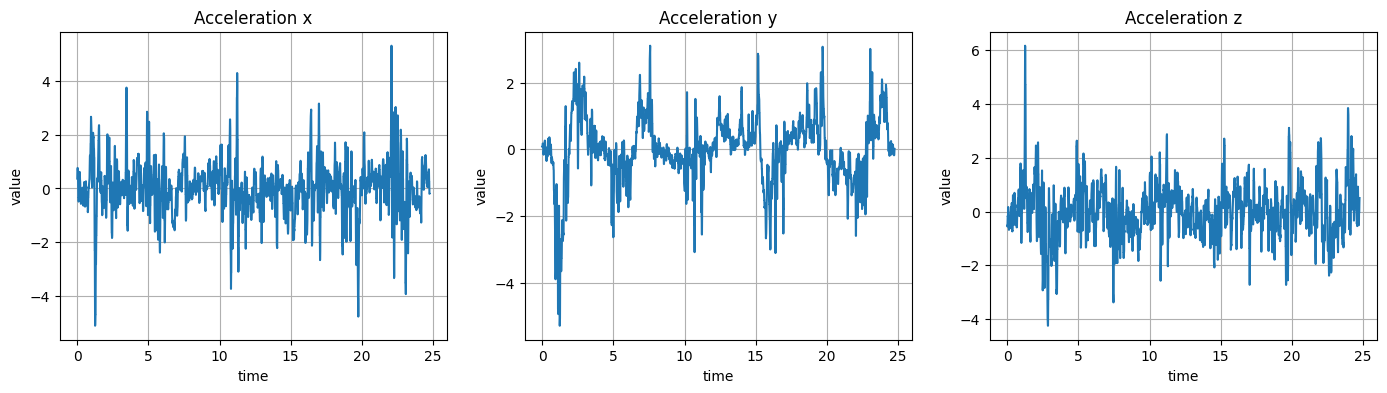
\includegraphics[width=1.0\linewidth]{imagens/ruido.png}

            \textbf{Fonte:} Autoria própria
            \label{fig:ruido}
        \end{figure}

        Observa-se pela figura que um algoritmo de filtragem é extremamente necessário para que se possa descrever o comportamento ideal das variáveis medidas. A linguagem de programação Python será usada previamente para implementação dos filtros por sua simplicidade e versatilidade, entretanto, os filtros selecionados serão posteriormente convertidos para código de máquina para implementação eficiente e embarcada. 
        
        \subsubsection{Espectro de Frequência}
            No contexto de filtros, o domínio da frequência é essencial para a realização eficaz do processo de filtragem. De modo geral, os dados brutos são convertidos para o domínio da frequência, onde os ruídos costumam se concentrar nas faixas de frequência mais altas \hyperlink{WRIGHT}{(WRIGHT, 2024)}. Um algoritmo é então responsável por limitar os dados de frequência a um intervalo específico, sendo a frequência máxima desse intervalo denominada frequência de corte ($f_c$). O gráfico a seguir (\autoref{fig:freq}) apresenta a implementação de um espectro de frequência em conjunto com um filtro padrão de alta ordem.

            \begin{figure}[H]
                \centering
                \caption{Diagrama de Frequência com Filtro}
                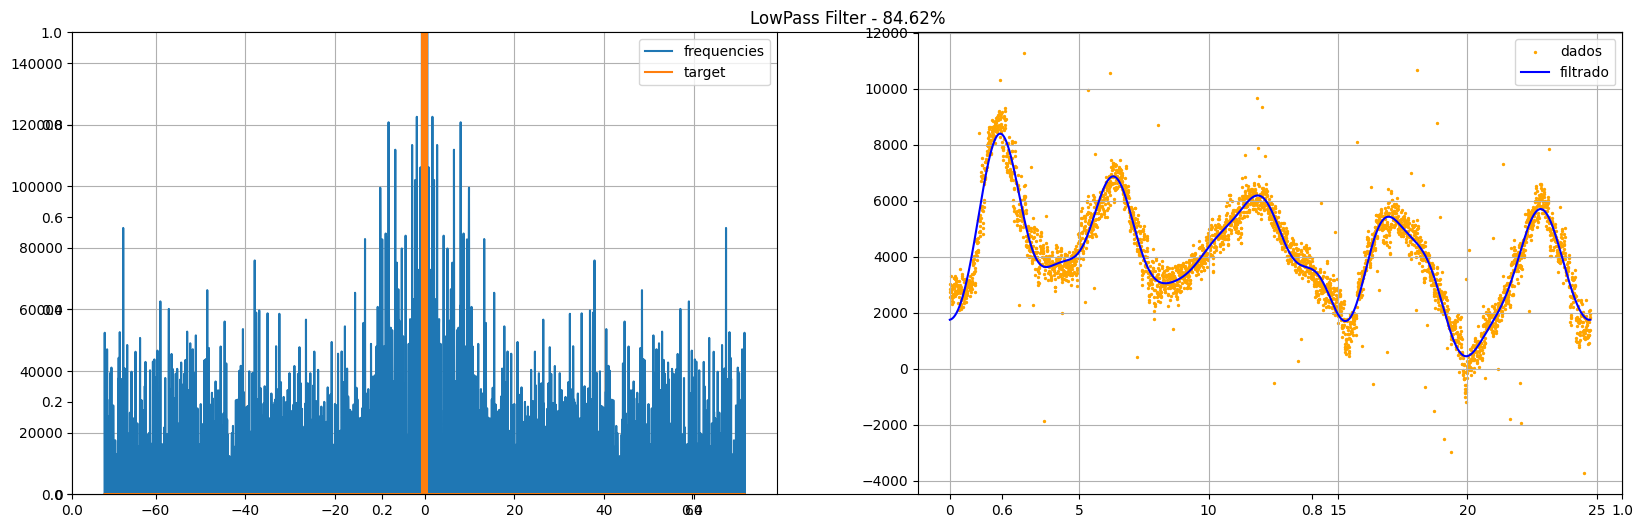
\includegraphics[width=1.0\linewidth]{imagens/frequencia.png}
    
                \textbf{Fonte:} Autoria própria
                \label{fig:freq}
            \end{figure}

            A partir da figura, observa-se que a maior parte das frequências está concentrada no intervalo de -20 a +20 Hz. Para impor uma alta restrição de frequência, foi adotada uma frequência de corte $f_c = 1$ Hz, resultando em um gráfico suavizado, compatível com o comportamento real do sistema. Nota-se que, quanto maior a frequência de corte, menor será a atuação do filtro sobre os dados. Por outro lado, uma frequência de corte muito baixa promove uma suavização excessiva, impedindo o acompanhamento de picos ou variações abruptas provenientes da resposta do sensor. Dessa forma, torna-se necessário definir um ponto de equilíbrio adequado para a escolha de $f_c$ (corte laranja no gráfico).

        \subsubsection{Filtro Passa Baixa de Segunda Ordem}
            O filtro passa-baixa foi implementado corretamente, conforme apresentado na \autoref{fig:freq}. Contudo, essa abordagem exigiu a coleta de todos os dados antes da eliminação das altas frequências, o que não é viável em sistemas embarcados, uma vez que os dados são adquiridos em tempo real e, portanto, devem ser filtrados de forma simultânea. Para atender a essa exigência, foi desenvolvido um filtro de segunda ordem, com base nos fundamentos teóricos da transformada de Laplace3 e do espectro de frequência, resultando na formulação de uma função de transferência de segunda ordem, dada por:

            \begin{equation}
                G(s) = \frac{\omega_n^2}{s^2 + 2\zeta\omega_n s + \omega_n^2}
            \end{equation}

            Onde $\zeta = \sqrt{2} = 0.7071$ para corte em $\omega_n = 2\pi f_c$. A função de transferência é então digitalizada e transformada em uma equação de diferenças a partir das entradas anteriores, que pode ser facilmente implementada em um microcontrolador de baixo processamento como um Arduino ou similar. Assim sendo, o gráfico da \autoref{fig:pass2} mostra a implementação desse filtro nos dados. Uma observação importante é que o programa deve alcançar um período de amostragem $dt$, definido a partir da capacidade do microcontrolador de coletar dados do sensor individualmente. 

            \begin{figure}[H]
                \centering
                \caption{Diagrama de Frequência com Filtro}
                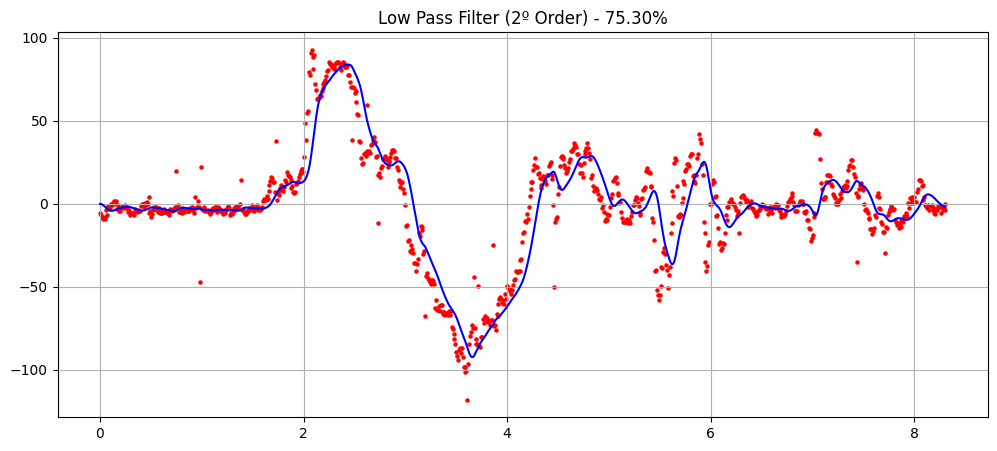
\includegraphics[width=.8\linewidth]{imagens/pass2.png}
    
                \textbf{Fonte:} Autoria própria
                \label{fig:pass2}
            \end{figure}

            Observa-se pelo gráfico que o filtro (linha azul) acompanha com grande precisão os dados brutos de inclinação evitando outliers. 

            \subsubsection{Filtro de Kalman}
                O filtro de Kalman é um algoritmo recursivo de estimação que permite inferir o estado mais provável de um sistema dinâmico ao longo do tempo, mesmo que as medições estejam sujeitas a ruído e incertezas \hyperlink{UFF}{(UFF, 2017)}. Ele é amplamente usado em áreas como controle, navegação, fusão de sensores, finanças e robótica. O equacionamento deste filtro é dado a partir de matrizes, onde coeficientes de ajuste e parametrização do filtro é informado ().
    
                \begin{center}
                \centering       
                \addtocounter{table}{-1}
                \scriptsize
                \vspace{-0.3cm}
            
                {\renewcommand{\arraystretch}{2.2}
                \begin{longtable}{|c|c|c|c|}
                    \caption{\small Parâmetros do Filtro de Kalman} \label{tab:parametros_kalman}\\
                    \hline
                        \fcol{1.5}{\textbf{Parâmetro}} & 
                        \col{3.2}{\textbf{Tipo / Unidade}} & 
                        \col{5.2}{\textbf{Intuição prática (“tradução”)}} & 
                        \col{5.2}{\textbf{Como ajustar / escolher}} \\
                    \hline
                        \fcol{1.5}{$x_0$} & 
                        \col{3.2}{Escalar (mesma unidade)} & 
                        \col{5.2}{Palpite inicial do valor real} & 
                        \col{5.2}{Use a 1\textsuperscript{a} leitura do sensor mais confiável ou um valor médio} \\
                    \hline
                        \fcol{1.5}{$P_0$} & 
                        \col{3.2}{Escalar $\geq 0$ (unidade$^2$)} & 
                        \col{5.2}{Variância inicial $\rightarrow$ quão incerto você está sobre $x_0$} & 
                        \col{5.2}{Grande $\Rightarrow$ confia pouco no palpite; Pequeno $\Rightarrow$ confia muito} \\
                    \hline
                        \fcol{1.5}{$Q$} & 
                        \col{3.2}{Escalar $\geq 0$ (unidade$^2$)} & 
                        \col{5.2}{Ruído do modelo $\rightarrow$ permite que o estado mude entre amostras} & 
                        \col{5.2}{Aumente para reagir mais rápido; diminua para suavizar} \\
                    \hline
                        \fcol{1.5}{$R$} & 
                        \col{3.2}{Matriz $3 \times 3$ (diag)} & 
                        \col{5.2}{Ruído de medição de cada sensor ($\sigma^2$ na diagonal)} & 
                        \col{5.2}{Coloque $\sigma^2$ de cada sensor; maior $\sigma^2 \Rightarrow$ peso menor na fusão} \\
                    \hline
                \end{longtable}}
            
                \small
                \textbf{Fonte:} \href{https://tinyurl.com/2a54wjmx}{Autoria Própria}
            \end{center}

            O algoritmo de Kalman também será usado posteriormente para fusão de sensores e filtros diferentes. Pelo gráfico da \autoref{fig:kalman}, observa-se que o filtro acompanha os dados, assim como o anterior.
            
            \begin{figure}[H]
                \centering
                \caption{Diagrama de Frequência com Filtro}
                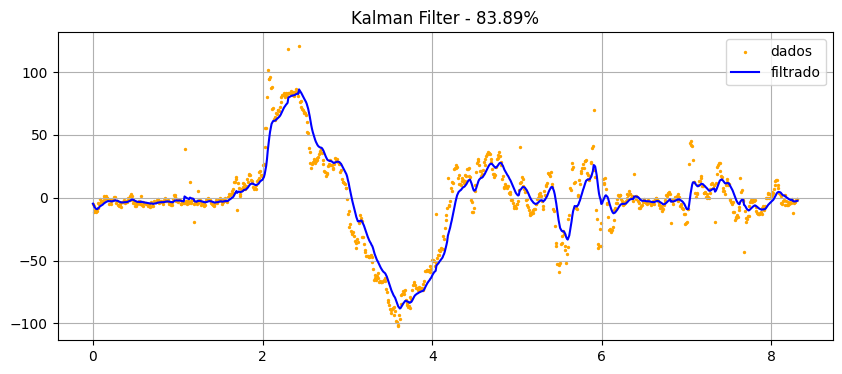
\includegraphics[width=.8\linewidth]{imagens/kalman.png}
    
                \textbf{Fonte:} Autoria própria
                \label{fig:kalman}
            \end{figure}

            Por se tratar de um filtro adaptativo, apresenta vantagens em relação a filtros convencionais, ao lidar de maneira mais eficaz e "inteligente"\ com erros acumulativos e variações abruptas, ajustando-se dinamicamente às condições do sinal.

        \subsubsection{Filtro de Média Móvel}
            Esse é um filtro simples e eficaz, que substitui cada ponto de dados pela média dos pontos em uma janela móvel de forma eficiente. O gráfico a seguir mostra a implementação desse filtro com uma janela de tempo de 20 posições.

            \begin{figure}[H]
                \centering
                \caption{Filtro de Média Móvel}
                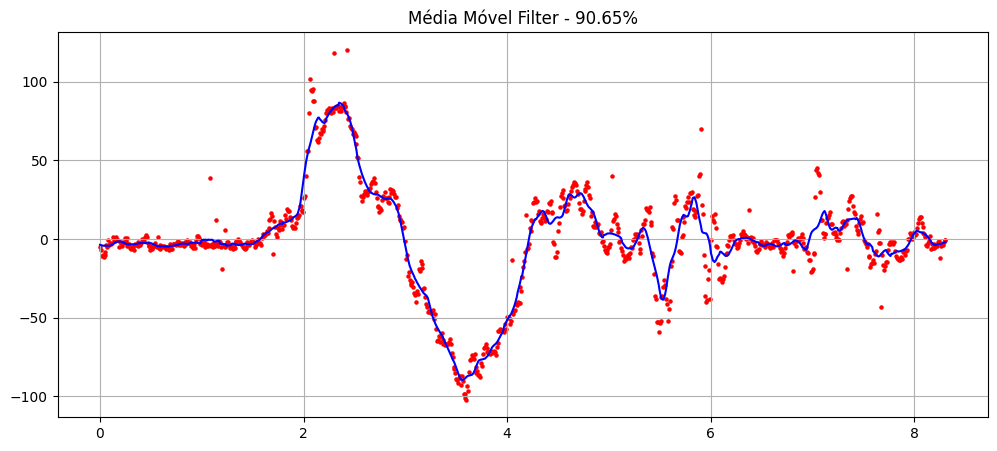
\includegraphics[width=.8\linewidth]{imagens/media.png}
    
                \textbf{Fonte:} Autoria própria
                \label{fig:kalman}
            \end{figure}

            Embora apresente simplicidade e facilidade de integração, o filtro possui como principal desvantagem a ausência de parametrização em função do espectro de frequência, exigindo ajuste manual da janela até que o comportamento desejado seja alcançado. Adicionalmente, observa-se aumento significativo na demanda por armazenamento conforme o tamanho da janela cresce, exigindo maior número de posições.

        \subsubsection{Filtro de Savitzky-Golay}
            Este filtro ajusta um polinômio de baixa ordem a uma janela deslizante de pontos de dados, preservando a forma geral dos dados (como picos e vales) enquanto suaviza o ruído. Ideal para preservar as características da curva. Diferentemente do filtro de média móvel, a saída é dada a partir de um polinômio que se adapta ao conjunto de dados em tempo real por interpolação, possibilitando maior precisão com uma menor janela de deslizamento.

            \begin{figure}[H]
                \centering
                \caption{Filtro de Savitzky-Golay}
                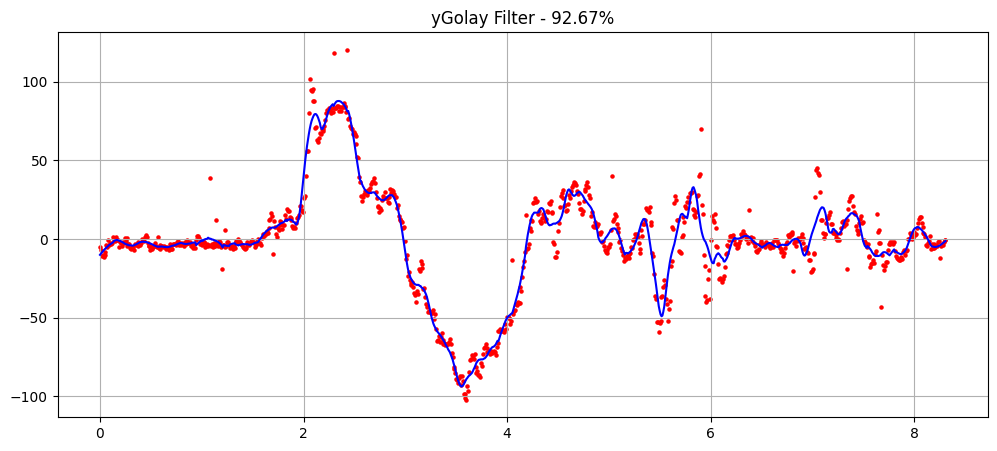
\includegraphics[width=.8\linewidth]{imagens/golay.png}
    
                \textbf{Fonte:} Autoria própria
                \label{fig:kalman}
            \end{figure}

            Este algoritmo, embora apresente desempenho superior em relação ao filtro simples de média móvel, demanda elevado poder de processamento e um consumo significativo de memória RAM para sua implementação, o que pode se tornar um fator limitante em sistemas baseados em microcontroladores com baixa capacidade de processamento.

        \subsubsection{Filtro Gaussiano}
            Esse filtro aplica uma função gaussiana aos dados em uma janela, o que resulta em uma suavização mais natural e contínua. Ele pode ser facilmente implementado informando o desvio padrão dos dados, o que pode ser obtida após uma análise anterior, ou em tempo real a partir de uma certa amostra. A \autoref{fig:gaus} mostra a implementação do algoritmo nos mesmos dados.

            \begin{figure}[H]
                \centering
                \caption{Filtro de Gaussiano}
                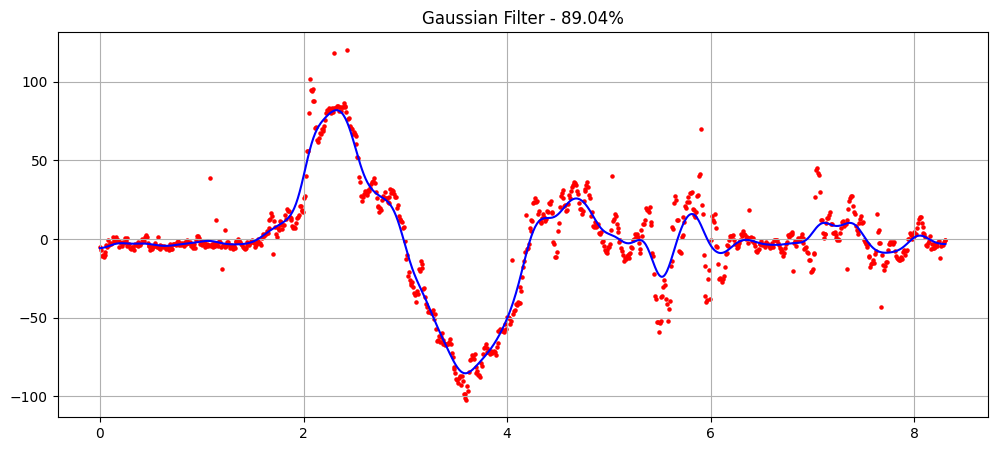
\includegraphics[width=.8\linewidth]{imagens/gauss.png}
    
                \textbf{Fonte:} Autoria própria
                \label{fig:gaus}
            \end{figure}

            Este filtro também usa uma janela de dados e apresenta as mesmas preocupações de processamento. Uma abordagem comum é usar a mesma janela para implementar os filtros semelhantes e a partir de uma média simples ou ponderada, encontrar um valor que condiz com a realidade das variáveis medidas.

        \subsubsection{Comparação Final}
            Os filtros apresentados neste documento correspondem aos mais analisados e implementados de forma prática. Outros filtros também foram avaliados, porém descartados após criteriosa análise. Esse processo permitiu a elaboração de um estudo comparativo, com o objetivo de identificar os filtros mais adequados para prosseguimento. Na próxima seção, os filtros selecionados serão combinados para a geração de uma saída final com maior precisão. A tabela a seguir apresenta a comparação entre os filtros avaliados.

            \begin{center}
                \centering 
                \scriptsize
                \vspace{-0.3cm}
            
                {\renewcommand{\arraystretch}{2.2}
                \begin{longtable}{|c|c|c|c|c|c|}
                    \caption{\small Estudo de Filtros} \label{tab:parametros_kalman}\\
                    \hline
                        \fcol{3}{\textbf{Filtro}} & 
                        \col{2}{\textbf{Categoria}} & 
                        \col{2}{\textbf{Velocidade de Resposta}} & 
                        \col{2}{\textbf{Suavização}} & 
                        \col{2.2}{\textbf{Complexidade Computacional}} & 
                        \col{3.2}{\textbf{Fonte}} \\
                    \hline
                        \fcol{3}{Média Móvel} & 
                        \col{2}{Suavização Temporal} & 
                        \col{2}{Lento} & 
                        \col{2}{Alta} & 
                        \col{2.2}{Média} & 
                        \col{3.2}{\href{https://amaruescalante.io/files/analysis-moving-average-imu-8-bit.pdf}{\textbf{AMARUESCALANTE}}} \\
                    \hline
                        \fcol{3}{Passa Baixa} & 
                        \col{2}{Frequencial} & 
                        \col{2}{Médio (customizável)} & 
                        \col{2}{Alta} & 
                        \col{2.2}{Alta} & 
                        \col{3.2}{\href{https://tinyurl.com/29dxq5rf}{\textbf{VECTORNAV}}} \\
                    \hline
                        \fcol{3}{Kalman} & 
                        \col{2}{Adaptativo (estatístico)} & 
                        \col{2}{Rápido} & 
                        \col{2}{Média}  & 
                        \col{2.2}{Média} & 
                        \col{3.2}{\href{https://tinyurl.com/2xlvfym5}{\textbf{BTRACK}}} \\
                    \hline
                        \fcol{3}{Savitzky-Golay} & 
                        \col{2}{Suavização (Polinomial)} & 
                        \col{2}{Médio} & 
                        \col{2}{Alta}  & 
                        \col{2.2}{Média} & 
                        \col{3.2}{\href{https://tinyurl.com/2xkgg4ep}{\textbf{WIKIPEDIA}}} \\
                    \hline
                        \fcol{3}{Gaussiano} & 
                        \col{2}{Suavização (Temporal)} & 
                        \col{2}{Médio} & 
                        \col{2}{Alta}  & 
                        \col{2.2}{Média} & 
                        \col{3.2}{\href{https://tinyurl.com/2ydj82rp}{\textbf{SPRINGPROFESSIONAL}}} \\
                    \hline
                        \fcol{3}{Butterworth} & 
                        \col{2}{Frequencial} & 
                        \col{2}{Médio} & 
                        \col{2}{Alta}  & 
                        \col{2.2}{Média} & 
                        \col{3.2}{\href{https://tinyurl.com/26carrqj}{\textbf{BLILEY}}} \\
                    \hline
                        \fcol{3}{Média Exponencial} & 
                        \col{2}{Suavização (IIR 1ª ordem)} & 
                        \col{2}{Médio} & 
                        \col{2}{Médio}  & 
                        \col{2.2}{Média} & 
                        \col{3.2}{\href{https://tinyurl.com/2ycxs3f4}{\textbf{VECTORNAV}}} \\
                    \hline
                \end{longtable}}
            
                \small
                \textbf{Fonte:} \href{https://tinyurl.com/2a54wjmx}{Anexo}
            \end{center}

        Com base nos estudos realizados, verificou-se que, mediante ajustes adequados nos filtros selecionados, é viável alcançar uma precisão satisfatória, com supressão quase integral dos principais ruídos identificados. Dentre os filtros analisados, destacaram-se como mais promissores o filtro de Kalman (amplamente empregado no setor), em conjunto com o filtro gaussiano, o filtro passa-baixa e o filtro de Butterworth. A correta combinação desses elementos promove uma melhoria substancial na confiabilidade e na suavização dos dados brutos adquiridos pelo sistema.
        
    \newpage
    \subsection{Fusão de Filtros}
        Devido à variedade de filtros existentes, com características específicas quanto ao tempo de resposta, capacidade de suavização e adaptação a novos dados, uma abordagem eficaz é a combinação desses filtros. Essa estratégia visa obter uma saída final que agregue as qualidades individuais, potencializando a precisão e aumentando a robustez do sistema. Diante disso, serão apresentados os métodos disponíveis para viabilizar tal combinação.
        \vspace{-0.3cm}

        \subsubsection{Convariance Intersection}
            A intersecção de covariância é uma técnica que garante que o sistema não fique excessivamente confiante ao combinar estimativas incertas de diferentes fontes \hyperlink{DINGLER}{(DINGLER, 2024)}. Antes de realizar a fusão por filtros, é preciso obter a incerteza nas medições de cada sensor. De modo geral isso é feito através do desvio padrão em uma distribuição gaussiana, utilizando a relação $\varDelta = k\,\sigma$.
            \vspace{-.15cm}
    
            \begin{itemize}
                \item Cerca de 68\% dos valores caem dentro de $\pm 1\sigma$ do valor médio, $k=1$\vspace{-.2cm}
                \item Cerca de 95\% caem dentro de $\pm 2\sigma$, $k=2$\vspace{-.2cm}
                \item Cerca de 99,7\% dentro de $\pm 3\sigma$, $k=3$
            \end{itemize}
            \vspace{-0.15cm}

            Com os dados brutos, o desvio padrão médio foi de $\sigma = 1853.94$. Adotando 68\% de confiança (para fins de teste), obtém-se a variância $P = \sigma^2 = 3437093.523$. Com isso, o algoritmo de convariance intersection pode ser encontrado com:
            \vspace{-0.15cm}
    
            \begin{itemize}
                \item x1, x2: estimativas escalares (valores de entrada)\vspace{-.2cm}
                \item p1, p2: variâncias (incerteza de medida)\vspace{-.2cm}
                \item w: parâmetro de fusão (confiança na entrada x1) $\Rightarrow$ valores entre [0, 1] (100\%)\vspace{-.2cm}
                \item Retorna (xf, pf): estimativa fundida e variância fundida
            \end{itemize}

            \noindent A \autoref{fig:ci_3filters} mostra a implementação desse algoritmo a partir da junção de 3 filtros.

             \begin{figure}[H]
                \centering
                \caption{Fusão de Filtros por CI}
                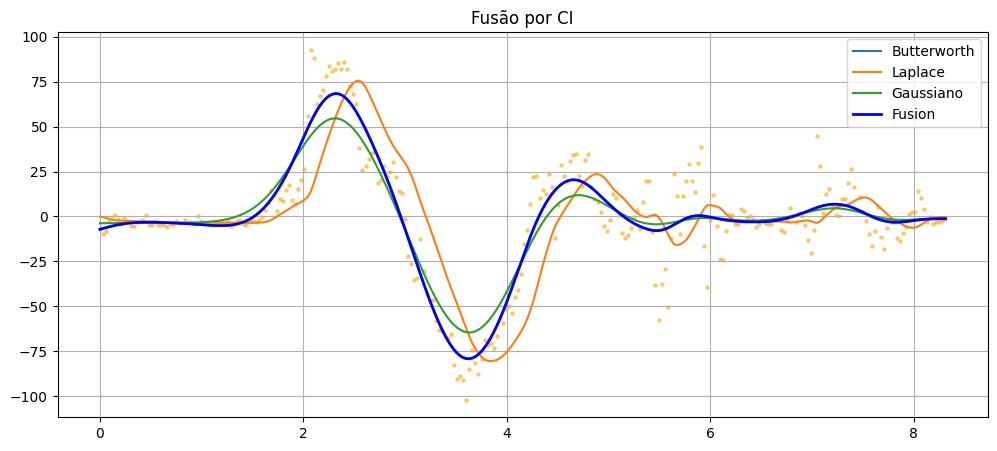
\includegraphics[width=.8\linewidth]{imagens/ci.png}
    
                \textbf{Fonte:} Autoria própria
                \label{fig:ci_3filters}
            \end{figure}
            
        \subsubsection{Fusão por Kalman}
            O método de Covariance Intersection apresenta semelhanças com o algoritmo e o filtro de Kalman, uma vez que também utiliza as variáveis com base na confiança atribuída a cada dado a ser fundido, resultando em uma saída única e adaptativa. Ressalta-se, contudo, que sua implementação difere substancialmente de abordagens baseadas em médias simples ou ponderadas. Essa distinção confere ao método maior precisão, ao considerar filtros com diferentes comportamentos dinâmicos, tempos de assentamento, níveis de confiabilidade, entre outros parâmetros. A fusão realizada incorpora essas variáveis para gerar uma estimativa otimizada. O gráfico da \autoref{fig:falman_fusion} ilustra o comportamento resultante da aplicação desse método.

            \begin{figure}[H]
                \centering
                \caption{Fusão de Filtros por Kalman}
                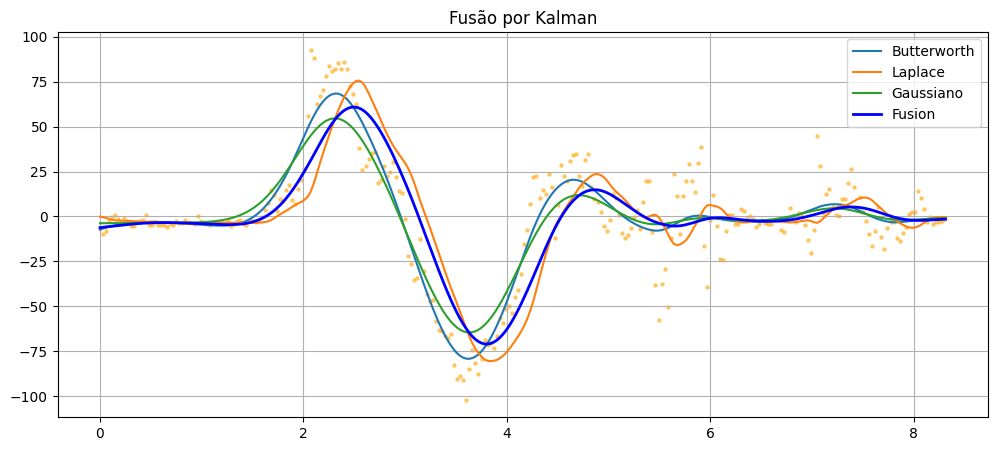
\includegraphics[width=.8\linewidth]{imagens/kalman_fusion.png}
    
                \textbf{Fonte:} Autoria própria
                \label{fig:falman_fusion}
            \end{figure}

            Uma limitação do método apresentado, comum também a outras abordagens clássicas, é a exigência de um conhecimento detalhado das especificações tanto dos filtros quanto dos sensores utilizados. Esse nível de compreensão é necessário para realizar múltiplas simulações e combinações, com o objetivo de identificar a parametrização mais adequada para os dados. Ademais, considerando que os próprios sensores, sujeitos a erros inerentes, constituem a principal ferramenta de medição, torna-se inviável a comparação com uma curva de referência ou resposta ideal. Dessa forma, o processo de parametrização tende a ser conduzido de maneira empírica, baseado em tentativa e erro.

        \newpage
        \subsubsection{Aprendizagem de Máquina}
            A limitação discutida na seção anterior pode ser contornada por meio da adoção de uma abordagem alternativa nos métodos de fusão de sensores, utilizando técnicas avançadas de aprendizagem de máquina. Com crescente relevância nos últimos anos, essas técnicas baseiam-se na aplicação de algoritmos de inteligência artificial capazes de identificar relações diretas entre variáveis de entrada e a saída desejada, proporcionando elevada capacidade de adaptação a diferentes contextos. Nesse cenário, propõe-se o uso das saídas dos filtros, bem como de seus históricos, como variáveis de entrada do modelo. Quanto maior o número de dados anteriores considerados, maior a tendência de acurácia do sistema. A saída ideal, por sua vez, deve ser previamente monitorada e empregada como referência para o comportamento que o sistema deverá replicar.

            \begin{figure}[H]
                \centering
                \caption{Comparação de Modelos Machine Learning}
    
                \subfloat[Modelo com Regressão Linear]{
                    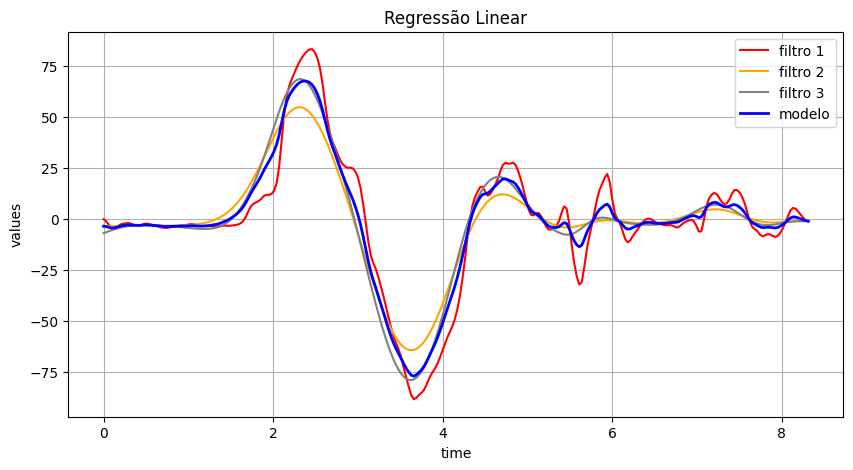
\includegraphics[width=0.48\linewidth]{imagens/model_linear.png}
                }\hfill
                \subfloat[Modelo com Random Forest]{
                    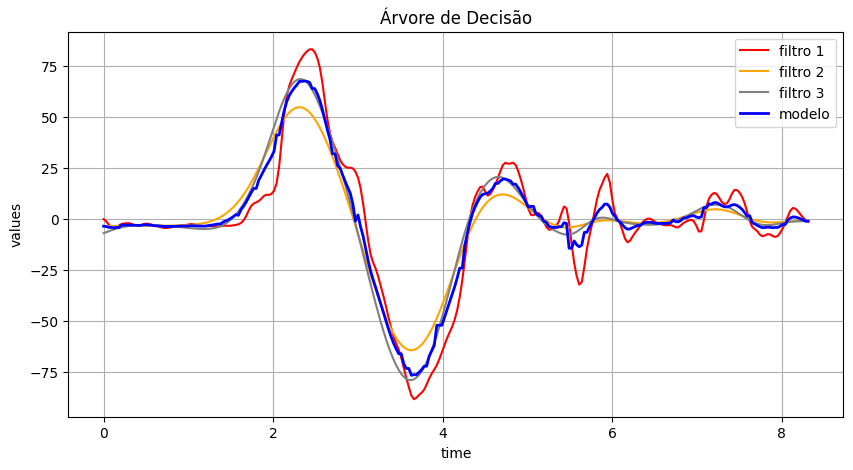
\includegraphics[width=0.48\linewidth]{imagens/model_random.png}
                }
                
                \subfloat[Modelo com Gradient Booster]{
                    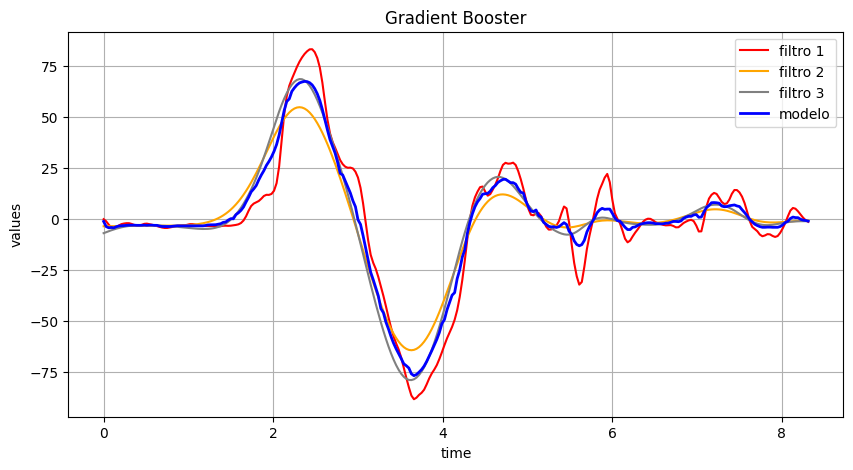
\includegraphics[width=0.55\linewidth]{imagens/model_gradient.png}
                }
                
                \label{fig:all_models}
                \textbf{Fonte:} Autoria Própria
            \end{figure}
            
            A Figura\autoref{fig:all_models} apresenta a comparação entre diferentes algoritmos de machine learning, com o propósito de prever a saída ideal a partir dos valores anteriores de três filtros distintos. Para fins de teste, definiu-se como referência a média simples das saídas dos filtros. O objetivo da análise consistiu em avaliar a capacidade dos modelos em aproximar-se da saída desejada de forma eficiente e consistente.

            A análise dos gráficos demonstrou que todos os modelos avaliados foram capazes de acompanhar a saída desejada com elevado desempenho, atingindo 100\% de precisão na comparação entre os dados de treinamento e teste. Esses resultados indicam, com elevado grau de confiança, que algoritmos de inteligência artificial podem ser utilizados para combinar saídas de sensores menos precisos ou filtros com limitações específicas, de modo a gerar uma estimativa mais robusta e confiável. 
            
            A saída-alvo pode, inclusive, corresponder à resposta de um sensor de alta precisão empregado em aplicações industriais, viabilizando uma melhoria significativa na qualidade dos dados apenas por meio de software. Contudo, essa abordagem impõe maior demanda computacional, exigindo processadores mais potentes para lidar com algoritmos de machine learning que utilizam um grande volume de variáveis, como os 100 últimos valores de 10 filtros distintos. Caso essa estratégia seja implementada com sucesso, é possível reduzir significativamente os custos do projeto, promovendo uma calibração mais acessível e eficiente dos sensores.

    \newpage
    \subsection{Fusão de Sensores}
        Alternativamente à fusão direta a partir dos filtros, é viável aplicar filtros individualmente aos sensores e realizar a fusão posteriormente. Para isso, foram utilizados dois módulos contendo acelerômetro e giroscópio: o MPU6050 e o MPU9250, os quais apresentam diferenças em termos de escala, tempo de resposta e nível de ruído. A proposta consiste em normalizar os dados provenientes de ambos os sensores, de modo a adequá-los à mesma escala, e, em seguida, aplicar algoritmos de fusão com o objetivo de obter uma saída unificada e mais precisa do que aquelas fornecidas isoladamente por cada sensor.

        \subsubsection{Filtragem Antes}
            Uma das abordagens utilizadas para a filtragem dos dados consiste na aplicação de filtros individuais em cada sensor antes da execução do algoritmo de fusão. Para isso, foram implementados filtros passa-baixa distintos em cada sensor, considerando tempos de assentamento e ultrapassagem diferenciados, em função das características específicas de resposta de cada dispositivo. Posteriormente, as saídas filtradas foram combinadas por meio do método Covariance Intersection, resultando em uma única estimativa consolidada.
            
            \begin{figure}[H]
                \centering
                \caption{Fusão de Sensores Antes da Filtragem}
                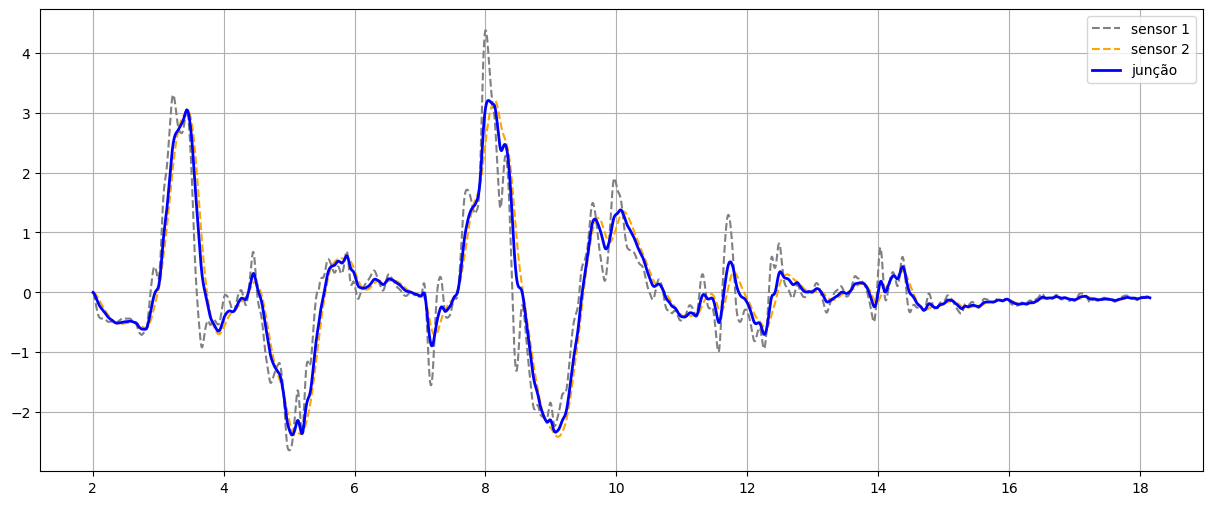
\includegraphics[width=.8\linewidth]{imagens/fusion_sensors_antes.png}
    
                \textbf{Fonte:} Autoria própria
                \label{fig:ci}
            \end{figure}

            Verifica-se que a saída final tende a representar um valor intermediário entre os dois sensores, apresentando comportamento aparentemente superior ao de cada sensor isoladamente, com uma resposta mais suavizada. No entanto, essa abordagem implica um aumento no custo computacional, uma vez que a introdução de um filtro adicional antecede a etapa de fusão, acrescentando uma operação extra ao processamento.

        \subsubsection{Filtragem Depois}
            Ao aplicar a filtragem apenas na saída final, o sistema de fusão assume a responsabilidade de gerar uma estimativa única a partir dos dados brutos de cada sensor, realizando a filtragem em uma única etapa ao término do processo. Essa abordagem reduz o custo computacional ao eliminar a necessidade de múltiplas filtragens. A \autoref{fig:ci2} apresenta o resultado final obtido após a fusão e posterior filtragem.
            
            \begin{figure}[H]
                \centering
                \caption{Fusão de Sensores Após a Filtragem}
                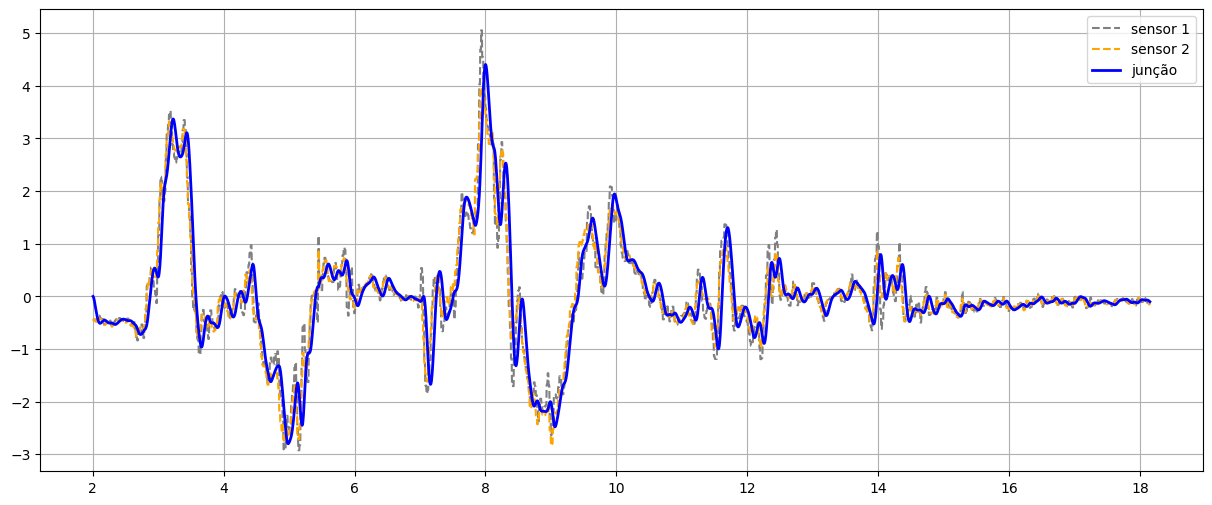
\includegraphics[width=.8\linewidth]{imagens/fusion_sensors_depois.png}
    
                \textbf{Fonte:} Autoria própria
                \label{fig:ci2}
            \end{figure}

            Embora o comportamento geral seja semelhante, observa-se um nível de ruído mais elevado em comparação ao gráfico anterior. Isso ocorre porque o filtro final não leva em consideração as particularidades individuais de cada sensor, exigindo que o software realize a parametrização da saída com base em um sinal já afetado pelo ruído. Ademais, em situações nas quais apenas um dos sensores apresenta ruído em determinado instante, o algoritmo de fusão pode gerar uma estimativa final distorcida, ainda que não se trate de uma simples média, o que pode resultar em erros de medição.
        
        \subsubsection{Modelo de Aprendizagem de Máquina}
            De modo análogo aos modelos de machine learning previamente desenvolvidos, é possível implementar uma abordagem baseada na utilização de valores passados dos sensores, permitindo a comparação com uma referência ou saída desejada. No entanto, essa estratégia implica em maior custo computacional, pois o próprio algoritmo de aprendizagem deve incorporar uma etapa de filtragem interna para acompanhar a curva de referência. As figuras a seguir ilustram a variação da acurácia do modelo em função do aumento da quantidade de valores anteriores considerados na predição do próximo valor.
            
            \begin{figure}[H]
                \centering
                \caption{Comparação de Modelos Machine Learning}
    
                \subfloat[Modelo de Fusão (1 valores anteriores)]{
                    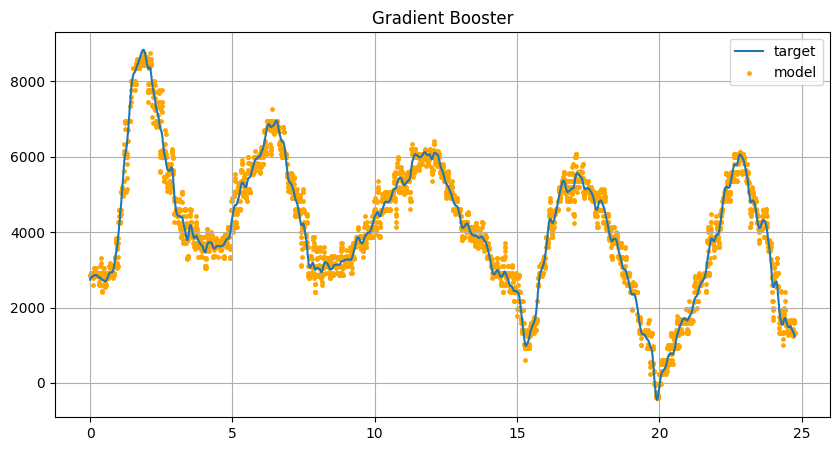
\includegraphics[width=0.48\linewidth]{imagens/gb1.png}
                }\hfill
                \subfloat[Modelo de Fusão (5 valores anteriores)]{
                    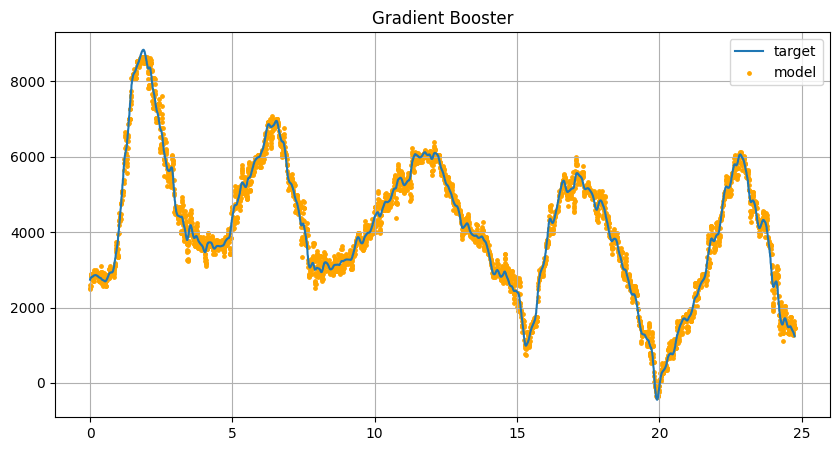
\includegraphics[width=0.48\linewidth]{imagens/gb5.png}
                }
                
                \subfloat[Modelo de Fusão (10 valores anteriores)]{
                    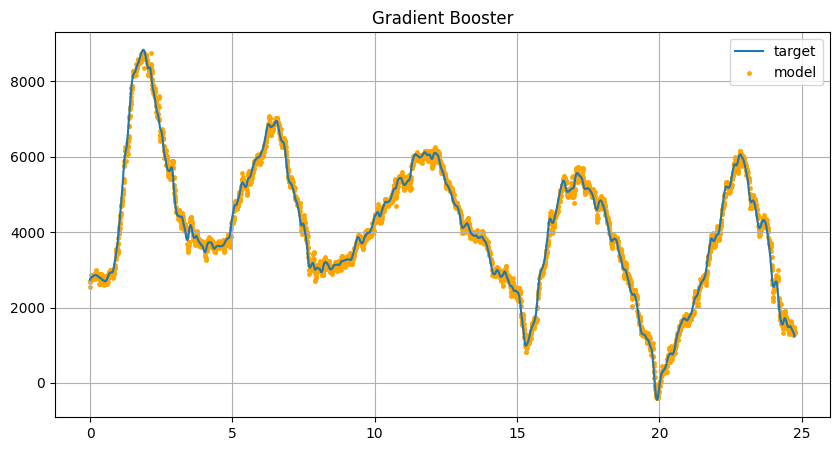
\includegraphics[width=0.48\linewidth]{imagens/gb10.png}
                }\hfill
                \subfloat[Modelo de Fusão (50 valores anteriores)]{
                    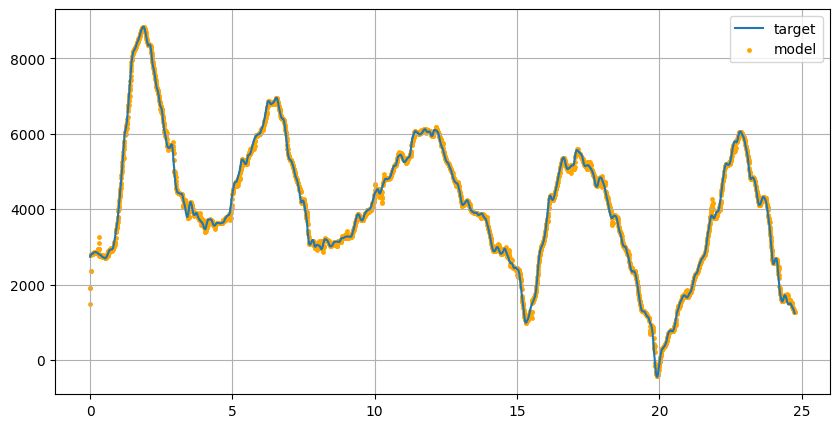
\includegraphics[width=0.48\linewidth]{imagens/gb50.png}
                }
                
                \label{fig:model2}
                \textbf{Fonte:} Autoria Própria
            \end{figure}

            Verifica-se que o modelo é capaz de seguir a curva de referência, neste caso, representada por um dos filtros utilizados para fins de teste, ainda que com a presença de leve ruído. Com base nos resultados obtidos, uma estratégia mais robusta consistiria na combinação das diferentes abordagens avaliadas. Nessa configuração, as entradas do modelo seriam compostas por dados brutos, sinais já filtrados, saídas dos algoritmos de fusão e variáveis derivadas, todas baseadas nos últimos $n$ valores observados, a fim de predizer o valor subsequente. Ressalta-se, contudo, a necessidade de dispor de uma referência confiável, ou seja, dados provenientes de um sensor de maior precisão, para aumentar a confiabilidade do modelo preditivo.

    \newpage
    \subsection{Inferência de Variáveis}
        A formulação matemática das variáveis de interesse, como posição, inclinação, velocidade linear e angular, possui relevância equivalente à medição direta dessas grandezas por sensores. Por meio dessas relações, torna-se viável a inferência de outras variáveis, reduzindo a necessidade de aquisição de sensores específicos e, consequentemente, os custos associados. 
        
        Ademais, a estimativa indireta de variáveis pode atuar como mecanismo de redundância ou aprimoramento da precisão, uma vez que permite a obtenção dos mesmos valores por diferentes métodos, exclusivamente via software. A \autoref{fig:3d} apresenta uma representação tridimensional elaborada pela equipe, ilustrando a posição de uma partícula em três eixos e destacando as principais variáveis espaciais, com o objetivo de facilitar a compreensão do sistema analisado.

        \begin{figure}[H]
            \centering
            \caption{Entendimento das Coordenadas em 3D}
            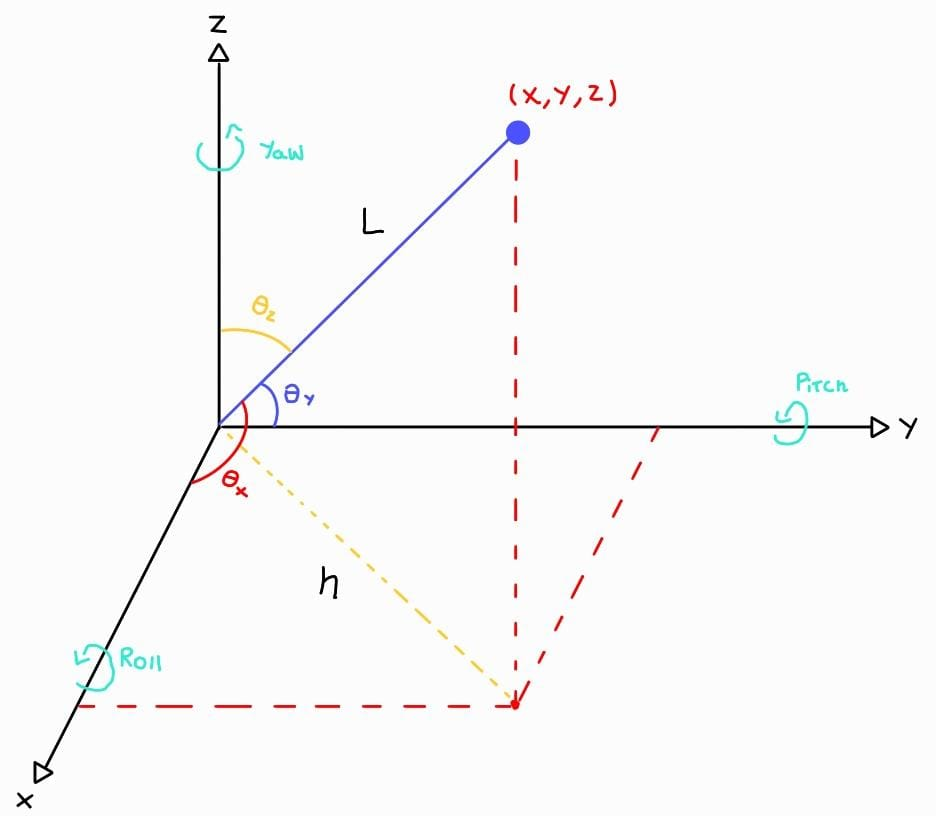
\includegraphics[width=.7\linewidth]{imagens/grafico.jpeg}

            \textbf{Fonte:} Autoria própria
            \label{fig:3d}
        \end{figure}

        A partícula localiza-se na posição definida pelo vetor $\hat{x} = (x, y, z)$ no sistema de coordenadas cartesianas, apresentando uma inclinação representada por $\hat{\theta} = (\theta_x, \theta_y, \theta_z)$ em relação aos respectivos eixos. Essa configuração está conectada à origem, definida por $\hat{x}_0 = (0, 0, 0)$, por uma distância absoluta $L$. As rotações em torno dos eixos $x$, $y$ e $z$, denominadas respectivamente como \textit{roll}, \textit{pitch} e \textit{yaw}, serão determinadas com base nas variáveis primárias do sistema \hyperlink{TAWIL}{(TAWIL, 2023)}.

        \subsubsection{Integração da Aceleração}
            A \autoref{fig:ruido}, apresentada na seção anterior, exibe a aceleração linear nos três eixos e será utilizada como base para a derivação de outras variáveis. Inicialmente, é necessário submeter esses dados a um filtro passa-faixa, a fim de isolar o intervalo de frequência que corresponde ao movimento dinâmico da partícula \hyperlink{EIBENSTEIN}{(EIBENSTEIN, 2017)}. Esse procedimento elimina componentes de baixa frequência, associadas à aceleração estática causada pela gravidade, bem como ruídos de alta frequência, considerados indesejáveis. Como resultado, preserva-se apenas a aceleração dinâmica, essencial para os cálculos subsequentes. O intervalo de frequência adequado foi determinado de forma empírica, sendo ilustrado no gráfico seguinte (Figura\autoref{fig:bora}), o qual apresenta tanto a faixa de frequência selecionada quanto os valores resultantes após a filtragem.

            \begin{figure}[H]
                \centering
                \caption{Filtragem e Análise dos Dados de Aceleração}
    
                \subfloat[Diagrama de Frequência]{
                    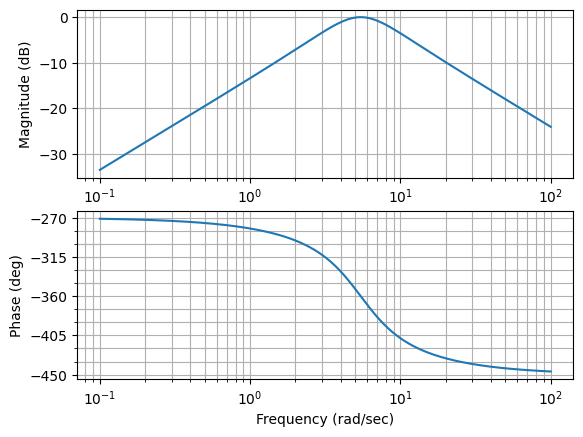
\includegraphics[width=0.48\linewidth]{imagens/banda.png}
                    \label{fig:freqa}
                }\hfill
                \subfloat[Gráfico de Atenuação de Frequência]{
                    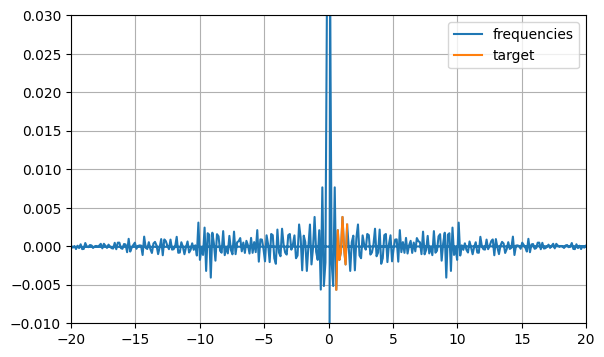
\includegraphics[width=0.48\linewidth]{imagens/bandb.png}
                }
                
                \subfloat[Valores de Aceleração Filtrados]{
                    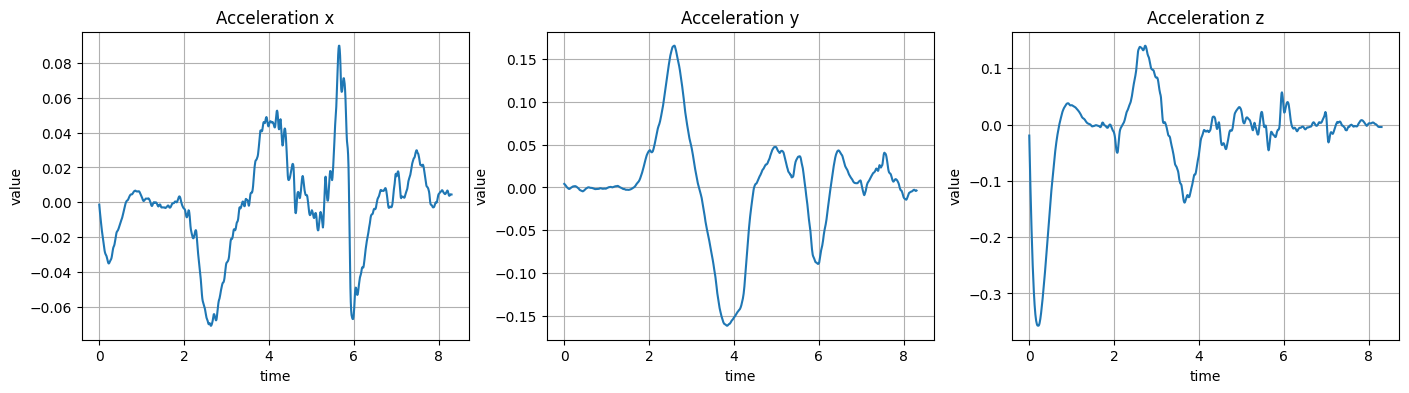
\includegraphics[width=0.96\linewidth]{imagens/bandc.png}
                }
                
                \label{fig:bora}
                \textbf{Fonte:} Autoria Própria
            \end{figure}

            Na Figura \ref{fig:nova}, verifica-se que as frequências não atenuadas concentram-se nas proximidades do pico, enquanto os valores fora desse intervalo são significativamente reduzidos, promovendo a filtragem e eliminação de componentes indesejadas. O resultado do processo corresponde à aceleração dinâmica, a qual será empregada nos cálculos subsequentes. A próxima variável a ser encontrada é a própria velocidade do sistema, que se dá pela relação da \autoref{eq:vel} a partir de integração \hyperlink{NATIONAL INSTRUMENTS}{(NATIONAL INSTRUMENTS, 2024)}.

            \vspace{-.15cm}\vspace{-.15cm}
            \begin{equation}
                a = \frac{dv}{dt} 
                \espaco\espaco\Rightarrow\espaco\espaco
                v = \int_{t_0}^t a(t)\,dt
                \label{eq:vel}
            \end{equation}

            A integração foi realizada por meio da Transformada de Laplace, aplicando-se à integral a correspondente função de transferência. A partir dessa representação contínua, utilizaram-se algoritmos de discretização para obtenção de uma equação de diferenças, viabilizando a implementação da solução em tempo real. Essa abordagem apresenta baixa complexidade computacional, sendo adequada para execução em plataformas embarcadas com recursos limitados, como microcontroladores. A \autoref{fig:velocidade} mostra o gráfico da velocidade a inferida a partir da aceleração por integração.

            \begin{figure}[H]
                \centering
                \caption{Valores de Velocidade Inferidos}
                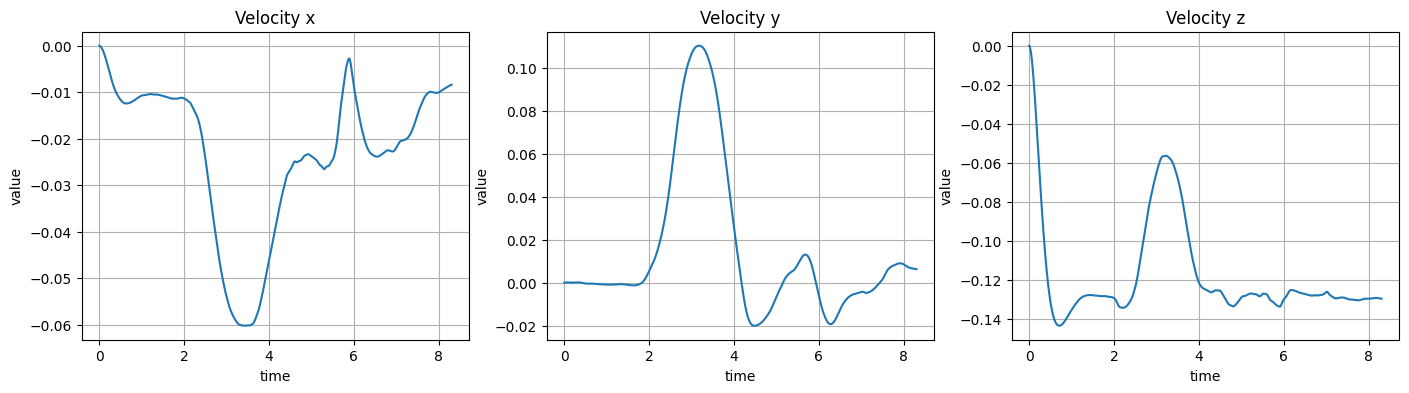
\includegraphics[width=\linewidth]{imagens/velocidade.png}
    
                \textbf{Fonte:} Autoria própria
                \label{fig:velocidade}
            \end{figure}\vspace{-.15cm}\vspace{-.15cm}

            A posição se dá da mesma forma e pode ser obtida através de uma nova integração a partir da velocidade por conta da relação presente na \autoref{eq:posint}.

            \vspace{-.15cm}
            \begin{equation}
                v = \frac{dx}{dt} \Rightarrow x = \int_{t_0}^t v(t)\,dt = \int_{t_0}^t \int_{t_0}^t a(t)\,dt\,dt
                \label{eq:posint}
            \end{equation}

            \noindent O gráfico da \autoref{fig:posicao} mostra o resultado da segunda integração.

            \begin{figure}[H]
                \centering
                \caption{Valores de Posição Inferidos}
                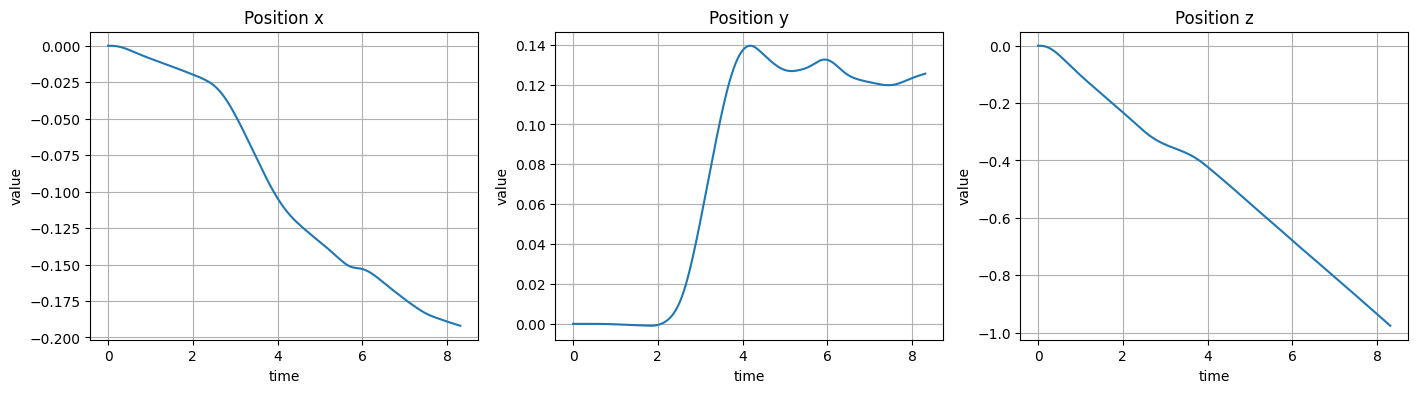
\includegraphics[width=\linewidth]{imagens/posicao.png}
    
                \textbf{Fonte:} Autoria própria
                \label{fig:posicao}
            \end{figure}

        \subsubsection{Integração da Inclinação}
            De forma similar, a inclinação também foi estimada pela integração das velocidades (desta vez, angular) $\hat{\omega} = (\omega_x, \omega_y, \omega_z)$, resultando nos ângulos $\hat{\theta} = (\theta_x, \theta_y, \theta_z)$. Antes da integração, aplicou-se um filtro passa-baixa aos dados brutos, visando eliminar ruídos de alta frequência, já que a gravidade não afeta significativamente essas componentes. A Figura\autoref{fig:nova} apresenta o diagrama de frequência utilizado para definir a faixa de corte do filtro.
             
            \begin{figure}[H]
                \centering
                \caption{Filtragem e Análise dos Dados de Inclinação}
    
                \subfloat[Diagrama de Frequência]{
                    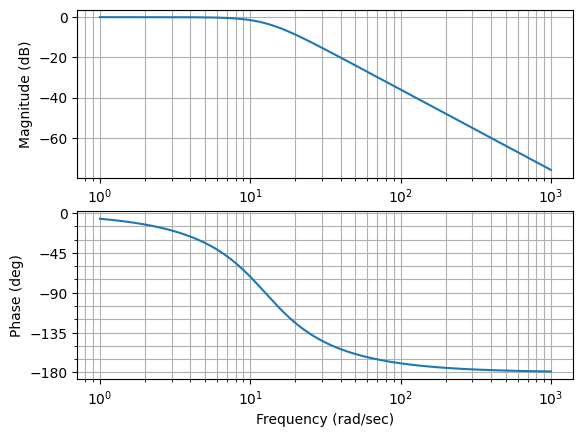
\includegraphics[width=0.48\linewidth]{imagens/low_a.png}
                    \label{fig:freqa}
                }\hfill
                \subfloat[Gráfico de Atenuação de Frequência]{
                    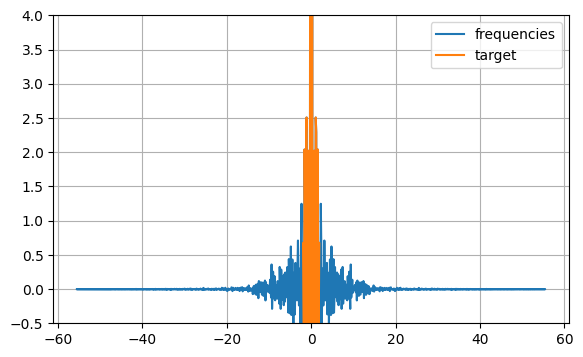
\includegraphics[width=0.48\linewidth]{imagens/low_b.png}
                }
        
                \subfloat[Valores de Velocidade Angular Filtrados]{
                    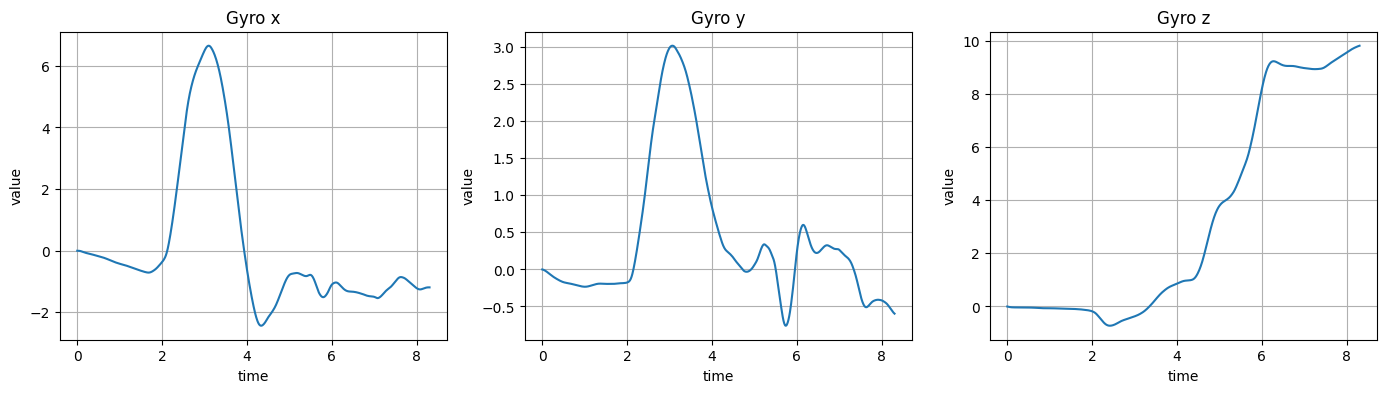
\includegraphics[width=0.96\linewidth]{imagens/low_d.png}
                }
                
                \subfloat[Valores de Inclinação Convertidos]{
                    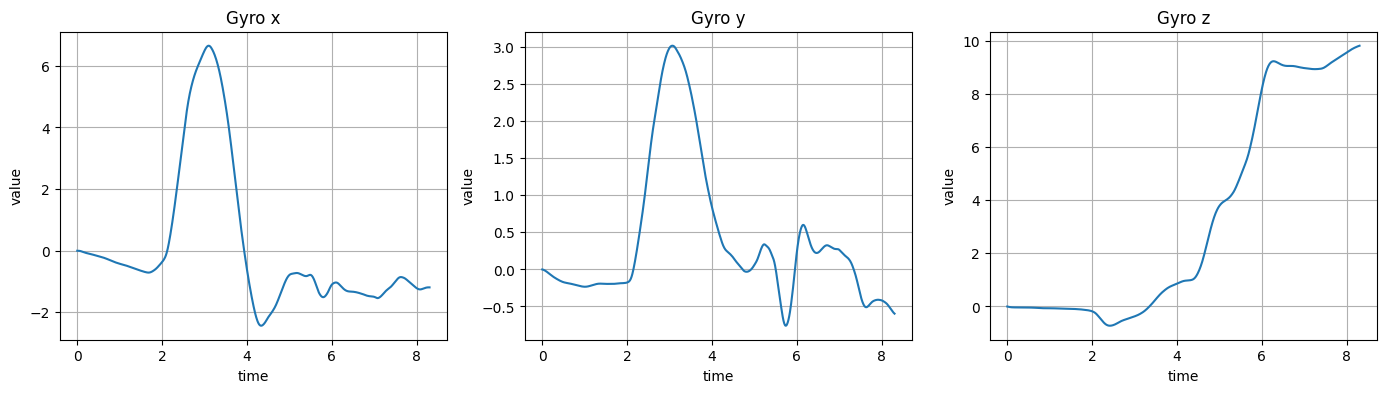
\includegraphics[width=0.96\linewidth]{imagens/low_d.png}
                }
                
                \label{fig:nova}
                \textbf{Fonte:} Autoria Própria
            \end{figure}

            

        \newpage
        \subsubsection{Projeção 3D}
            Com as coordenadas espaciais já determinadas, torna-se viável a construção de um gráfico tridimensional para avaliar se a trajetória do sensor corresponde à realidade física em três dimensões. Tal representação possibilita não apenas a análise da trajetória ao longo do tempo, mas também a visualização dos vetores de velocidade, permitindo identificar, por meio de uma representação vetorial, a direção e a intensidade do movimento em cada instante, sendo esta última expressa pela magnitude do vetor \hyperlink{MATHWORKS}{(MATHWORKS, 2025)}. A Figura\autoref{fig:3d_vet_a} apresenta a representação espacial tanto no plano bidimensional $xy$ quanto no espaço tridimensional. A mesma abordagem foi aplicada à inclinação, no gráfico subsequente.

            \vspace{-.15cm}
            \begin{figure}[H]
                \centering
                \caption{Posição Vetorial da Partícula}
    
                \subfloat[Plano $xy$]{
                    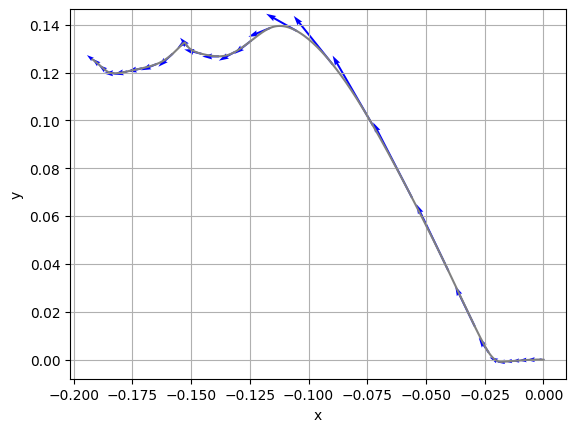
\includegraphics[height=6cm]{imagens/3da.png}
                    \label{fig:freqa_3d}
                }\hfill
                \subfloat[Plano $xyz$]{
                    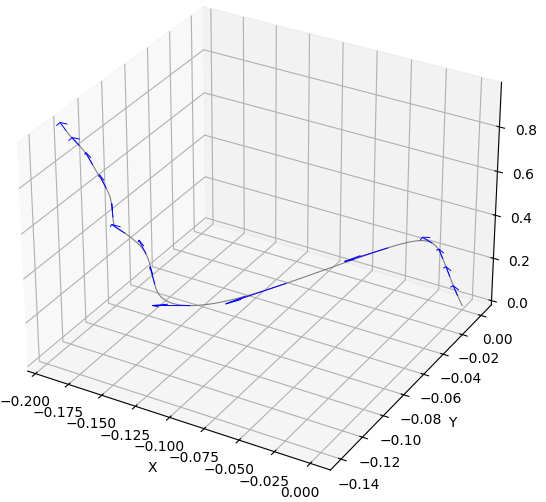
\includegraphics[height=6.6cm]{imagens/3db.png}
                }
                
                \label{fig:3d_vet_a}
                \vspace{-0.3cm}
                \textbf{Fonte:} Autoria Própria
            \end{figure}
            \vspace{-0.4cm}

            \begin{figure}[H]
                \centering
                \caption{Inclinação Vetorial da Partícula}
    
                \subfloat[Plano $xy$]{
                    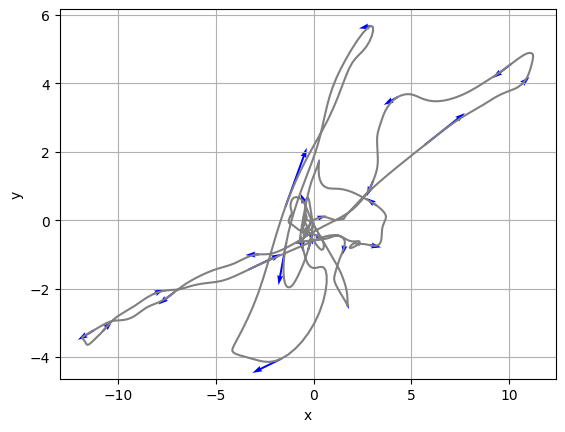
\includegraphics[height=6.3cm]{imagens/theta_3d_a.png}
                    \label{fig:vector_3d_a}
                }\hfill
                \subfloat[Plano $xyz$]{
                    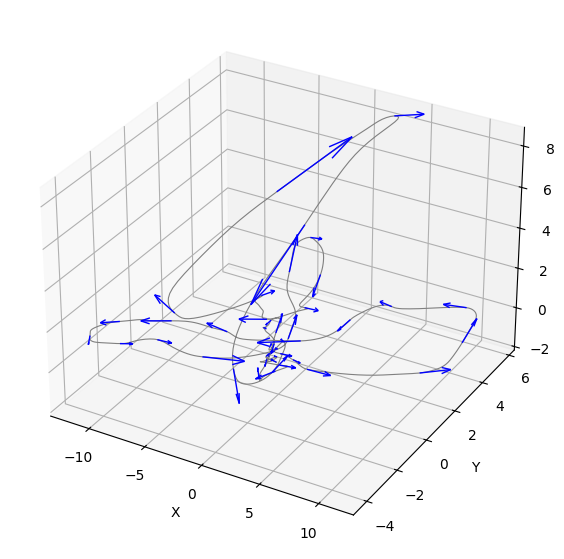
\includegraphics[height=6.6cm]{imagens/theta_3d_b.png}
                }

                \vspace{-0.3cm}
                \label{fig:freqaceel}
                \textbf{Fonte:} Autoria Própria
            \end{figure}
        
        \newpage
                
        \subsubsection{Pitch, Roll, Yaw}
            Os conhecimentos previamente adquiridos podem ser integrados para a obtenção das variáveis de interesse, especificamente as rotações acumuladas ao longo dos três eixos cartesianos, conforme ilustrado na \autoref{fig:3d}. Com base nos estudos conduzidos sobre o tema, verificou-se que a abordagem mais adequada para determinar tais variáveis a partir dos dados do acelerômetro e do giroscópio é por meio do uso de \textbf{quaternions}. Trata-se de uma representação matemática empregada principalmente na descrição de rotações em três dimensões \hyperlink{SCIELO}{(SCIELO, 2020)}, representado por:
            \vspace{-0.4cm}

            \begin{equation}
                q = q_0 + q_1i + q_2j + q_3k = (q_0, q_1, q_2, q_3)
            \end{equation}

            Onde $q_0$ é a parte escalar e $(q_1, q_2, q_2)$ formam o vetor tridimensional (parte imaginária). Os quaternions são usados para representar rotação sem ambiguidade (evitam o gimbal lock), interpolar suavemente entre rotações (SLERP), calcular rotações compostas de forma eficiente. A partir dele, é possível encontrar as demais variáveis: 
            
            \begin{equation}
                Pitch = arcsin\bigg(\,clamp\big(\,2(q_0q_2-q_3q_1), \,\,\,_{-1}, \, _1\,)\,\big)\bigg)
            \end{equation}
            
            \begin{equation}
                Roll = arctan2\bigg(\frac{2\cdot(q_0q_1 + q_2q_3)}{1-2(q_1^2 + q_2^2)}\bigg)    
            \end{equation}

            \begin{equation}
                Yaw = arctan2\bigg(\frac{2\cdot(q_0q_3 + q_1q_2)}{1-2(q_2^2 + q_3^2)}\bigg)    
            \end{equation}
            \vspace{-.3cm}

            O próximo passo consiste em encontrar o próprio vetor quaternion $q$, que pode ser obtido através de diferentes formas com diferentes precisões e tempos de resposta com respectivos erros associados. Em IMUs o padrão é realizar uma fusão de diferentes tipos de quartis (obtidos a partir de aceleração e de velocidade angular) e partir do acelerômetro e do giroscópio \hyperlink{STANFORD}{(STANFORD, 2019)}, dado por:
            \vspace{-0.3cm}

            \begin{equation}
                q = fusion(q_a, q_\omega)
            \end{equation}

            Onde $q_a$ é o quaternion obtido a partir do vetor aceleração $\textbf{a} = (a_x, a_y, a_z)$ e $q_\omega$ é obtido a partir das velocidade angulares $\omega = (0, \omega_x, \omega_y, \omega_z)$. De forma generalizada, o resultado será $q = (q_0, q_1, q_2, q_3)$.

            \vspace{.4cm}
            \noindent\ponto A partir da velocidade angular. 
            \vspace{-.5cm}
            
            \begin{equation}
                q_\omega = q_0 + \dot{q} \, dt
            \end{equation}

            \begin{equation}
                \dot{q} = \frac{1}{2} \, q \otimes \omega  
            \end{equation}
            
            \begin{equation}
                q \otimes \omega =
                    \begin{bmatrix}
                    q_0 & -q_1 & -q_2 & -q_3 \\
                    q_1 & q_0 & -q_3 & q_2 \\
                    q_2 & q_3 & q_0 & -q_1 \\
                    q_3 & -q_2 & q_1 & q_0 \\
                    \end{bmatrix}
                    \begin{bmatrix}
                    0 \\
                    \omega_x \\
                    \omega_y \\
                    \omega_z \\
                    \end{bmatrix}
            \end{equation}

            Lembrando que ao final, deve-se normalizar $q_\omega$ com.

            \begin{equation}
                q_\omega = \bigg(\frac{(q_0, q_1, q_2, q_3)}{\sqrt{q_0^2 + q_1^2 + q_2^2 + q_3^2}}\bigg)
            \end{equation}

            \noindent\ponto A partir da aceleração, deve-se normalizar as acelerações.

            \begin{equation}
                a = (a_x, a_y, a_z) = \bigg(\frac{a_x}{\sqrt{a_x^2 + a_y^2 + a_z^2}}, \frac{a_y}{\sqrt{a_x^2 + a_y^2 + a_z^2}}, \frac{a_z}{\sqrt{a_x^2 + a_y^2 + a_z^2}}\bigg)
            \end{equation}

            \noindent E esses novos valores serão usados para as fórmulas abaixo.

            \begin{equation}
                q_a = q_{yaw} \otimes (q_{pitch} \otimes q_{roll})
            \end{equation}
    
            \begin{equation}
                q_{roll} = \left[ \cos\left(\frac{\phi}{2}\right), \; \sin\left(\frac{\phi}{2}\right), \; 0, \; 0 \right]
            \end{equation}

            \begin{equation}
                q_{pitch} = \left[ \cos\left(\frac{\theta}{2}\right), \; 0, \; \sin\left(\frac{\theta}{2}\right), \; 0 \right] 
            \end{equation}

            \begin{equation}
                q_{yaw} = \left[ \cos\left(\frac{\psi}{2}\right), \; 0, \; 0, \; \sin\left(\frac{\psi}{2}\right) \right]
            \end{equation}            

            \begin{equation}
                pitch = arctan2\bigg(\frac{-a_x}{\sqrt{a_y^2 + a_z^2}}\bigg)
                \,\,\,\,\,\,\,\,\,\,\,\,\,\,\,\,\,\,
                roll = arctan2\bigg(\frac{a_y}{a_z}\bigg)
            \end{equation}

        \vspace{.25cm}
        Caso não haja o magnetômetro, adota-se $\psi = 0$ (yaw). Para calcular o yaw (rotação em torno do eixo Z) a partir de um magnetômetro, utiliza-se o campo magnético como referência para o norte magnético \hyperlink{NPX}{(NPX, 2010)}, com $m = (m_x, m_y, m_z)$. Esse processo exige correção da inclinação (roll e pitch) do sensor, senão o cálculo será impreciso.
        \vspace{-0.5cm}
        
        \begin{align*}
            m_x' &= m_x \cdot \cos\theta + m_z \cdot \sin\theta \\
            m_y' &= m_x \cdot \sin\phi \cdot \sin\theta + m_y \cdot \cos\phi - m_z \cdot \sin\phi \cdot \cos\theta
        \end{align*}

        \begin{equation}
            yaw = arctan2\bigg(\frac{-m_y'}{m_x'}\bigg)
        \end{equation}

        
\newpage
\setcounter{section}{3}
\section{Eletrônica e Circuitos}
    A seguir, apresentam-se as principais ferramentas e componentes empregados na montagem do protótipo funcional inicial de um DDRM, com o objetivo de assegurar níveis adequados de precisão e robustez. Tal abordagem visa possibilitar a comparação com soluções concorrentes disponíveis no mercado, além de orientar futuras melhorias no sistema.

\subsection{Componentes Eletrônicos} 
    O circuito base será estruturado em três camadas principais. A primeira camada, destinada à comunicação, conterá os componentes responsáveis por assegurar uma tensão adequada às camadas subsequentes, além de incluir dispositivos para estabilização de corrente. A camada intermediária abrigará o microprocessador principal do sistema, o qual terá a função de receber, filtrar e processar os dados provenientes dos sensores, além de transmitir as informações ao meio externo. Devido à sua relevância, essa camada requer proteção e segurança adequadas. Por fim, a camada inferior será dedicada à integração dos sensores utilizados no projeto. Os componentes selecionados para a construção do circuito principal estão listados na tabela a seguir.

      \begin{table}[H]
    \centering
    \caption{\small Componentes Eletrônicos Utilizados no Protótipo}
    \label{tab:variaveiss}
    \vspace{-0.4cm}
    \small
    {\renewcommand{\arraystretch}{1.5}
        \begin{longtable}{|c|c|c|c|}
        \hline
            \fcol{5.0}{\textbf{Componente}} &
            \col{3.8}{\textbf{Função}} &
            \col{1.6}{\textbf{Camada}} &
            \col{4.7}{\textbf{Fonte}} \\
        \hline
            \fcol{5.0}{Capacitor 0.68F}    &
            \col{3.8}{Estabilização} &
            \col{1.6}{3} &
            \col{4.7}{
                \href{https://www.powervolt.com.br/produtos/super-capacitor-goldcap-068f-55v-f-panasonic-eecrf0h684/}{POWER VOLT}
            } \\
        \hline
            \fcol{5.0}{Bateria 3650mah} &
            \col{3.8}{Estabilização} &
            \col{1.6}{3} &
            \col{4.7}{
                \href{https://tinyurl.com/26xqcpll}{MERCADO LIVRE}
            } \\
        \hline
            \fcol{5.0}{Raspeberry PI 4 Model B} &
            \col{3.8}{Processamento}  &
            \col{1.6}{2} &
            \col{4.7}{
                \href{https://tinyurl.com/239rpt7b}{AMAZON}
            } \\
        \hline
            \fcol{5.0}{MPU6050} &
            \col{3.8}{Sensoreamento}  &
            \col{1.6}{1} &
            \col{4.7}{
                \href{https://tinyurl.com/29r8mp6e}{PROESI}
            } \\
        \hline
            \fcol{5.0}{MPU9250} &
            \col{3.8}{Sensoreamento}  &
            \col{1.6}{1} &
            \col{4.7}{
                \href{https://tinyurl.com/28nqw52f}{ROBOCORE}
            } \\
        \hline
            \fcol{5.0}{ADXL335 } &
            \col{3.8}{Sensoreamento}  &
            \col{1.6}{1} &
            \col{4.7}{
                \href{https://tinyurl.com/2xjl4r35}{ROBO BUILDERS}
            } \\
        \hline
            \fcol{5.0}{Giroscópio HWT901B} &
            \col{3.8}{Sensoreamento (Alta Precisão)}  &
            \col{1.6}{1} &
            \col{4.7}{
                \href{https://pt.aliexpress.com/item/1005003003878184.html}{ALIEXPRESS}
            } \\
        \hline
            \fcol{5.0}{Acelerômetro GPS-IMU WTGAHRS3} &
            \col{3.8}{Sensoreamento (Alta Precisão)}  &
            \col{1.6}{1} &
            \col{4.7}{
                \href{https://pt.aliexpress.com/item/1005004002795311.html}{ALIEXPRESS}
            } \\
        \hline
            \fcol{5.0}{WitMotion HWT9053-485 ( } &
            \col{3.8}{Sensoreamento (Alta Precisão)}  &
            \col{1.6}{1} &
            \col{4.7}{
                \href{https://pt.aliexpress.com/item/1005003107175821.html}{ALIEXPRESS}
            } \\
        \hline
        \end{longtable}}
    \small
    \textbf{Fonte:} Autoria Própria
    \end{table}
    

\newpage
\subsection{Componentes Eletrônicos (consumo)}
        Antes do desenvolvimento da placa de circuito impresso (PCB), é imprescindível realizar a prototipagem do circuito, conectando os componentes eletrônicos por meio de jumpers e, quando viável, efetuando a soldagem em uma placa de fenolite. Essa etapa permite a verificação das interligações entre sensores e dispositivos, possibilitando ajustes precisos e, consequentemente, a redução de retrabalhos na versão final do circuito com a PCB concluída. A tabela a seguir apresenta os principais itens de consumo empregados durante o processo de prototipagem.
    
      \begin{table}[H]
        \centering
        \addtocounter{table}{-1}
        \caption{\small Componentes Consumo do Protótipo}
        \label{tab:variaveiss}
        \vspace{-0.4cm}
        \small
        {\renewcommand{\arraystretch}{1.5}
            \begin{longtable}{|c|c|c|c|}
            \hline
                \fcol{5.0}{\textbf{Componente}} &
                \col{3.8}{\textbf{Função}} &
                \col{1.6}{\textbf{Camada}} &
                \col{4.7}{\textbf{Fonte}} \\
            \hline
                \fcol{5.0}{Placa Fenolite Perfurada} &
                \col{3.8}{Integrar Componentes Eletrônicos}  &
                \col{1.6}{1}  &
                \col{4.7}{
                    \href{https://tinyurl.com/28c6jmeu}{ELETROGATE}
                } \\
            \hline
                \fcol{5.0}{Protoboard} &
                \col{3.8}{Prototipagem de Circuito}  &
                \col{1.6}{1, 2 e 3}  &
                \col{4.7}{
                    \href{https://tinyurl.com/27d3b7zk}{ELETROGATE}
                } \\
            \hline
                \fcol{5.0}{Cabo Flat 10 vias} &
                \col{3.8}{Comunicação Entre Dispositivos}  &
                \col{1.6}{1-2, 2-3}  &
                \col{4.7}{
                    \href{https://tinyurl.com/23c5tab9}{MAMUTE ELETRÔNICA}
                } \\
            \hline
                \fcol{5.0}{Pasta Solda} &
                \col{3.8}{Soldagem de Componentes}  &
                \col{1.6}{1 e 3}  &
                \col{4.7}{
                    \href{https://tinyurl.com/29qlg7dj}{MAGALU}
                } \\
            \hline
                \fcol{5.0}{Estanho de Solda} &
                \col{3.8}{Soldagem de Componentes}  &
                \col{1.6}{1, 2 e 3}  &
                \col{4.7}{
                    \href{https://tinyurl.com/22qekfnb}{LOJADOMECANICO}
                } \\
            \hline
                \fcol{5.0}{Malha Dessoldadora} &
                \col{3.8}{Soldagem de Componentes}  &
                \col{1.6}{-}  &
                \col{4.7}{
                    \href{https://tinyurl.com/2auu5pbw}{MRE FERRAMENTAS}
                } \\
            \hline
                \fcol{5.0}{Jumpers} &
                \col{3.8}{Prototipagem de Ligações}  &
                \col{1.6}{1, 2 e 3}  &
                \col{4.7}{
                    \href{https://tinyurl.com/24sj3zqd}{ROBOCORE}
                } \\
            \hline
            \end{longtable}}
        \small
        \textbf{Fonte:} Autoria Própria
        \end{table}

        A maioria dos componentes utilizados até o momento destina-se apenas à prototipagem, sendo prevista sua substituição gradual por elementos mais adequados às condições ambientais da plataforma, como capacitores com maior resistência à maresia. Contudo, considerando que o foco atual está na validação da funcionalidade dos algoritmos e na comunicação entre sensores e dispositivos, os componentes empregados atualmente são suficientes.

\newpage
\section{Placas de Circuito Impresso}
    O projeto requer avanços no software embarcado, especialmente na implementação de algoritmos que verifiquem se a configuração atual de sensores atinge taxa de amostragem superior a 50 Hz, compatível com o mercado. Diante disso, persiste a dúvida quanto ao uso de plataformas de prototipagem mais flexíveis, que permitem programação em MicroPython, com menor desempenho, ou dispositivos com maior capacidade de processamento, como o ESP32, programado em C++, porém com maior tempo de desenvolvimento e depuração. Assim, será adotada a construção de dois protótipos, um para cada microcontrolador e com linguagens distintas, visando facilitar a transposição de código entre plataformas, economizando tempo e evitando retrabalho caso uma das opções se mostre inviável.
    
\setcounter{section}{4}
\subsection{Circuitos Elétricos}
    O primeiro protótipo foi segmentado em quatro circuitos principais, cada qual com funções específicas. Entre os componentes utilizados, destacam-se os sensores MPU6050 e MPU9250, com acelerômetros e giroscópios embutidos, empregados nos testes iniciais dos algoritmos com o objetivo de avaliar a precisão e a eficiência do sistema em sua fase preliminar. A figura a seguir mostra cada um dos quarto subcircuitos que compõem o circuito geral, com os sensores e microcontroladores embarcados.

    \begin{figure}[H]
        \centering
        \caption{Circuitos Esquemáticos com Raspberry Pi PICO}
        
        \subfloat[Raspberry Pi Pico]{
            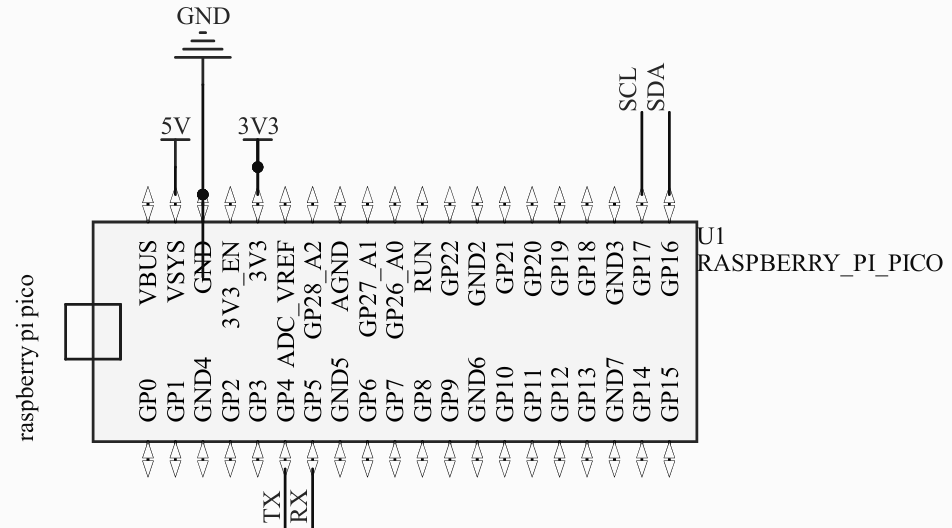
\includegraphics[height=4.5cm]{imagens/esq1a.png}
        }\hfill
        \subfloat[Sensores (MPU6050 e MPU9250)]{
            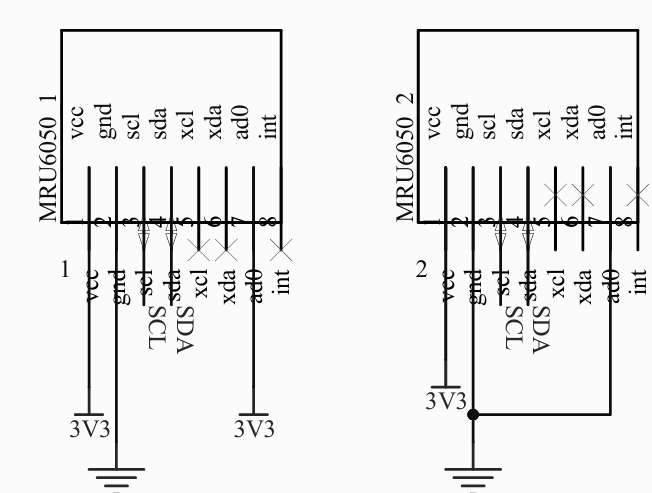
\includegraphics[height=4.5cm]{imagens/esq1b.png}
        }
        \newline
        \subfloat[Conector de 10 Vias]{
            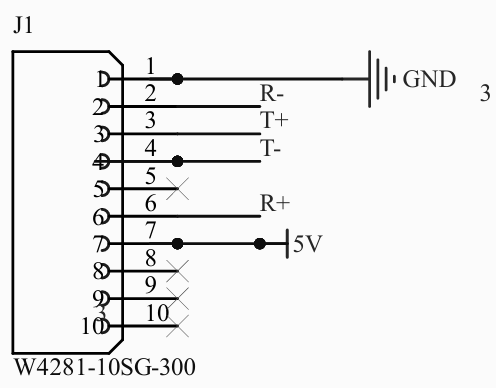
\includegraphics[height=4cm]{imagens/esq1c.png}
        }\hfill
        \subfloat[Módulo RS232]{
            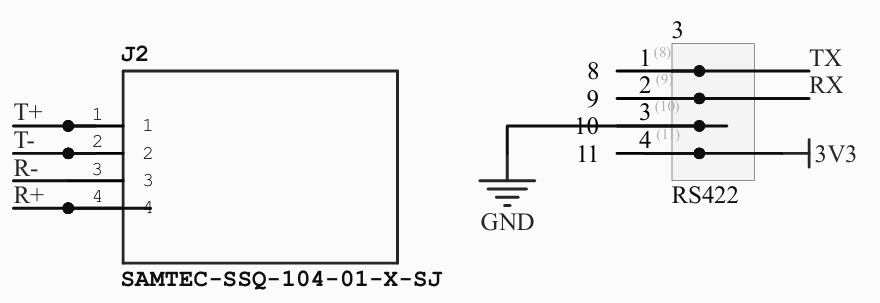
\includegraphics[height=3.5cm]{imagens/esq1d.png}
        }
        \label{fig:pcb1}

        \textbf{Fonte:} Autoria Própria
    \end{figure}

    O circuito utiliza como “cérebro” um Raspberry Pi Pico alimentado por 5V e regulado internamente a 3,3V, expondo até 30 GPIOs configuráveis para UART, I²C (SDA/SCL), ADC (GP26–28) e PWM, todas compartilhando o GND comum. Em paralelo, dois módulos de IMU MPU6050 (MPU-6050) ligados ao barramento I²C (SDA/SCL) e a dois pinos de interrupção distintos capturam acelerações e velocidades angulares, com pull-ups a 3,3 V e endereços independentes via AD0. A interface de campo conta com um conector de 10 vias W4281-10SG-300 que roteia sinais diferenciais RS-422 e fornece 5 V/GND para dispositivos externos. Por fim, um módulo RS-422 com driver/receptor diferencial converte o UART TTL do Pico (TX/RX a 3,3 V) em sinais T+/T- e R+/R– robustos para longa distância, mantendo referências de GND e 3,3 V. A Figura\autoref{fig:pcb2} mostra a mesma lógica aplicada ao segundo protótipo, alterando-se o microcontrolador para um ESP32 Dev Module.

    \begin{figure}[H]
        \centering
        \caption{Circuitos Esquemáticos com ESP32}
        
        \subfloat[ESP32]{
            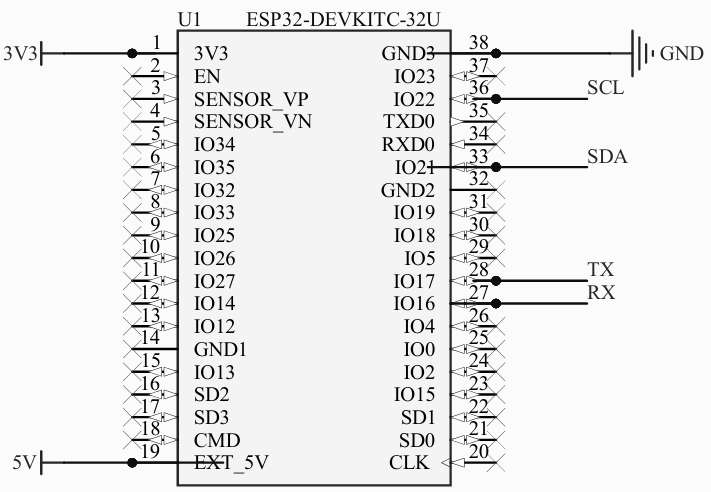
\includegraphics[height=4.5cm]{imagens/esq2a.png}
        }\hfill
        \subfloat[Sensores (MPU6050 e MPU9250)]{
            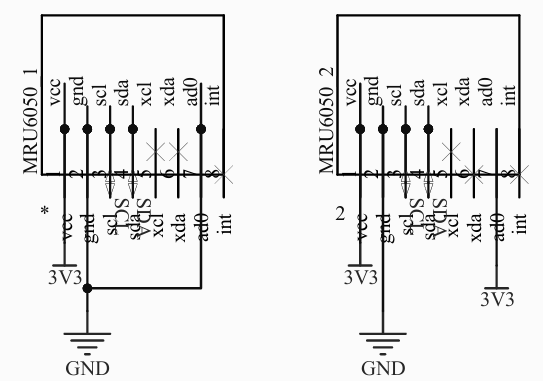
\includegraphics[height=4.5cm]{imagens/esq2b.png}
        }
        \newline
        \subfloat[Conector de 10 Vias]{
            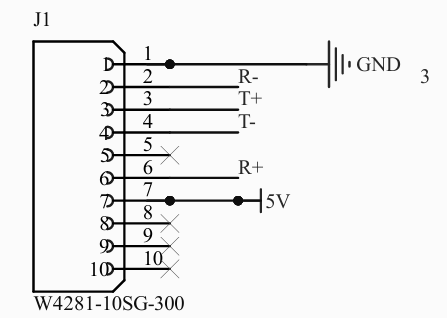
\includegraphics[height=4.3cm]{imagens/esq2c.png}
        }\hfill
        \subfloat[Módulo RS232]{
            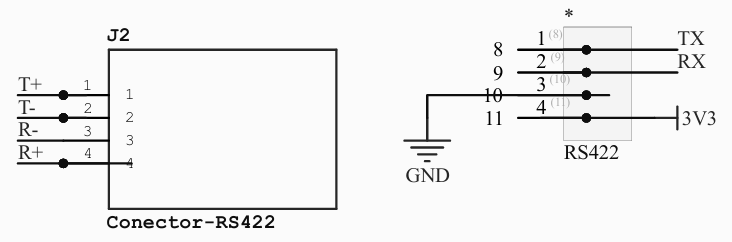
\includegraphics[height=3.3cm]{imagens/esq2d.png}
        }
        \label{fig:pcb2}

        \vspace{-0.2cm}
        \textbf{Fonte:} Autoria Própria
    \end{figure}

    \vspace{-0.1cm}
    A lógica de funcionamento é mantida no segundo protótipo, diferenciando-se unicamente pela utilização do ESP32 como microcontrolador central. Atuando nas mesmas faixas de operação de tensão, o circuito usa os mesmos sensores do primeiro protótipo, com grandes modificações no software embarcado. No momento, o desenvolvimento do código é realizado inicialmente em MicroPython no primeiro protótipo (com o Raspberry Pico), devido à maior facilidade de integração e depuração. Uma vez validada a funcionalidade, o código é transpilado para C++, a fim de explorar uma taxa de amostragem superior e maior capacidade de processamento.

    A adoção dessa abordagem apresenta como principal vantagem a possibilidade de transpilar e integrar o código entre diferentes plataformas com relativa facilidade, mesmo em caso de substituição do microcontrolador responsável pela gestão do sistema. Tal viabilidade decorre da similaridade entre as duas linguagens predominantes em sistemas embarcados. Essa compatibilidade proporciona à equipe maior autonomia para realizar testes exaustivos nos protótipos, assegurando que o projeto atenda aos requisitos estabelecidos e às exigências do mercado, com foco na robustez e confiabilidade do sistema.

\subsection{Placas de Circuito Impresso}
    Os dois microcontroladores foram selecionados na fase inicial do projeto em razão de sua versatilidade e confiabilidade em aplicações de sistemas embarcados. Devido à ampla adoção no mercado, esses dispositivos contam com suporte crescente, o que viabiliza a utilização de bibliotecas complementares que facilitam a implementação de algoritmos complexos, otimizando tempo e recursos. Com a integração dos componentes descritos na seção anterior, tornou-se possível a elaboração de uma placa de circuito impresso (PCI) geral, destinada à montagem dos protótipos iniciais do projeto. O primeiro protótipo corresponde aos circuitos ilustrados na Figura\autoref{fig:pcb1}, resultando na configuração final da PCI apresentada na Figura\autoref{fig:prot1a}.

    \begin{figure}[H]
        \centering
        \caption{Circuitos Esquemáticos com ESP32}
        
        \subfloat[PCB Final do Protótipo 01]{
            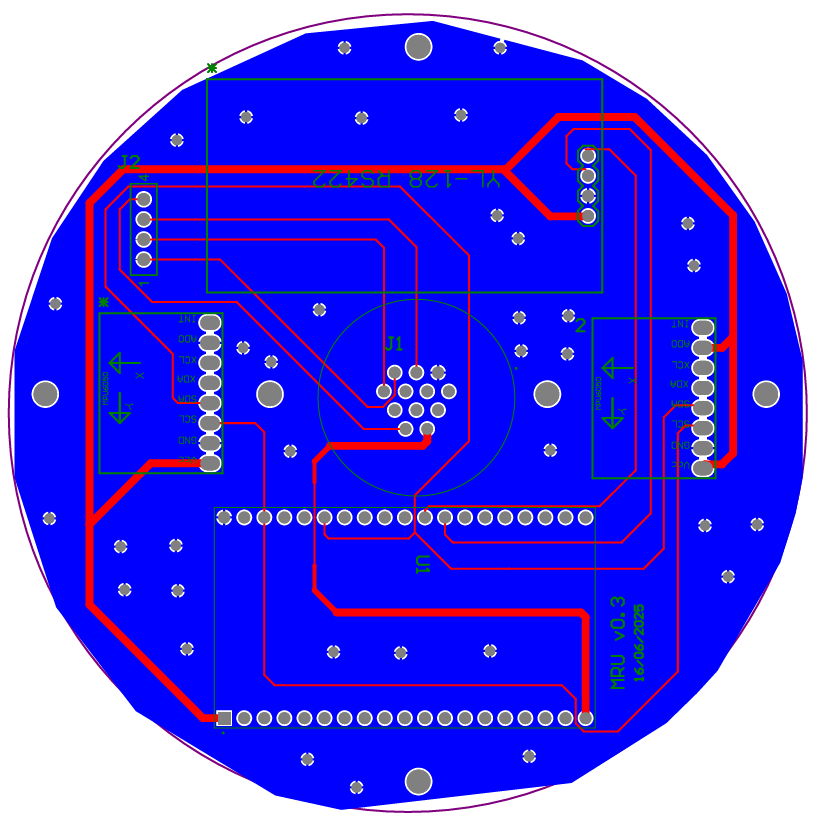
\includegraphics[width=7cm]{imagens/prot1.png}
            \label{fig:prot1a}
        }\hspace{.5cm}
        \subfloat[PCB Final do Protótipo 02]{
            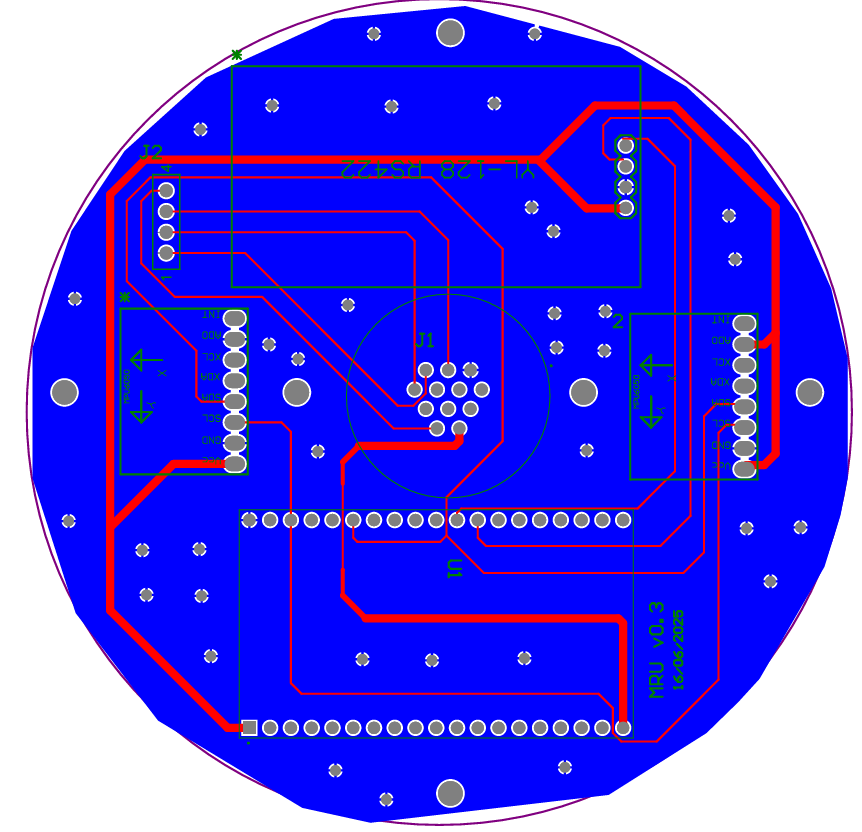
\includegraphics[width=7cm]{imagens/prot2.png}
            \label{fig:prot1b}
        }
        \label{fig:prot1}

        \textbf{Fonte:} Autoria Própria
    \end{figure}
    \vspace{-0.5cm}

    O mesmo princípio aplica-se ao protótipo 2, no qual o ESP32 é conectado à alimentação e aos sensores MPU6050 e MPU9250 por meio de duas trilhas destinadas à comunicação via protocolo I2C. Dessa forma, os sensores compartilham as mesmas vias de transmissão de dados, uma vez que operam em endereços distintos, o que permite a economia de recursos e a otimização do sistema para a integração de sensores adicionais. Essa abordagem evita a necessidade de fios e trilhas individuais para cada componente, prevenindo a sobrecarga do sistema. A Figura\autoref{fig:prot1b} apresenta o segundo protótipo, com implementações semelhantes às do primeiro.


     As duas placas descritas estão representadas em três dimensões nas figuras a seguir, proporcionando melhor visualização dos componentes e das trilhas que os interligam. É possível observar os dois sensores conectados e o microcontrolador principal, que pode ser acoplado ou removido externamente ao circuito.
    
    \begin{figure}[H]
        \centering
        \caption{PCB 3D do Protótipo com Raspberry Pi PICO}
        
        \subfloat[PCB Lado Frontal]{
            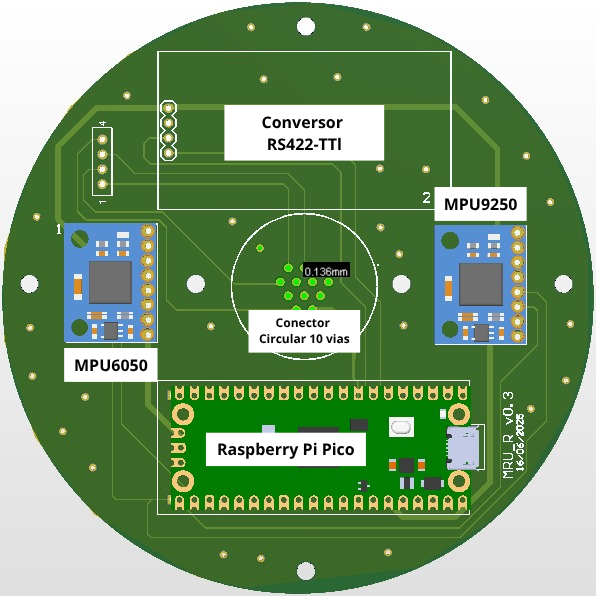
\includegraphics[height=7.2cm]{imagens/circ1a.png}
        }\hspace{.5cm}
        \subfloat[PCB Lado Traseiro]{
            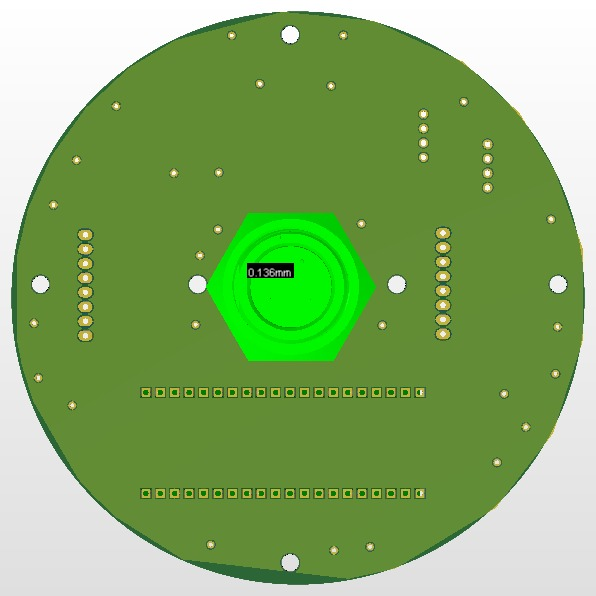
\includegraphics[height=7.2cm]{imagens/circ1b.jpg}
        }
        
        \label{fig:pcb1}
        \textbf{Fonte:} Autoria Própria
    \end{figure}
    \vspace{-0.5cm}

    \begin{figure}[H]
        \centering
        \caption{PCB 3D do Protótipo com ESP32}
        
        \subfloat[PCB Lado Frontal]{
            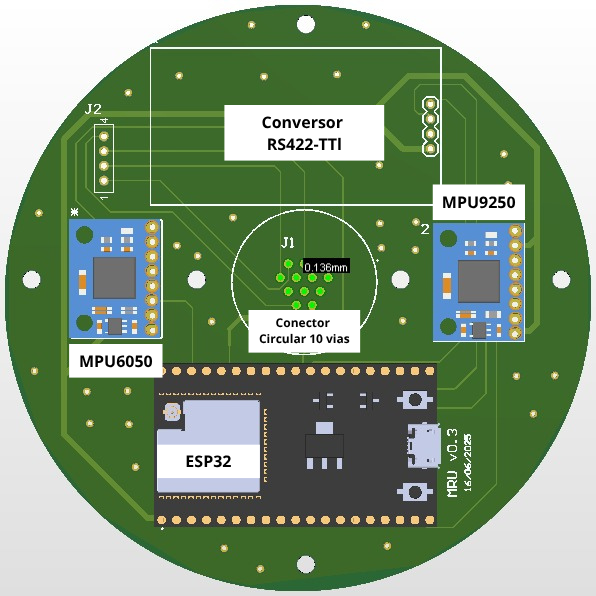
\includegraphics[height=7.2cm]{imagens/circ2a.png}
        }\hspace{.5cm}
        \subfloat[PCB Lado Traseiro]{
            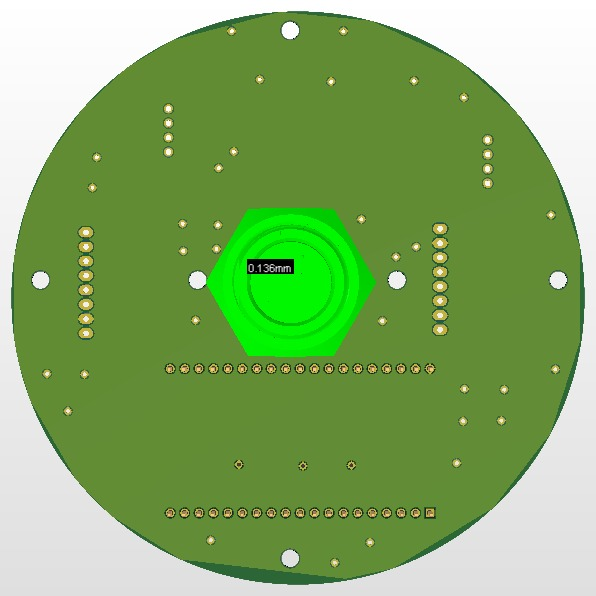
\includegraphics[height=7.2cm]{imagens/circ2b.jpg}
        }
        
        \label{fig:pcb1}
        \textbf{Fonte:} Autoria Própria
    \end{figure}

   O modelo tridimensional das PCBs de ambos os protótipos foi rotacionado, permitindo a visualização por diferentes ângulos. Essa abordagem visa ampliar a análise estrutural das placas para fins de desenvolvimento, conforme ilustrado nas figuras a seguir.

   \vspace{1cm}

   \begin{figure}[H]
        \centering
        \caption{PCB 3D do Protótipo 01}
        
        \subfloat[PCB Lado Frontal]{
            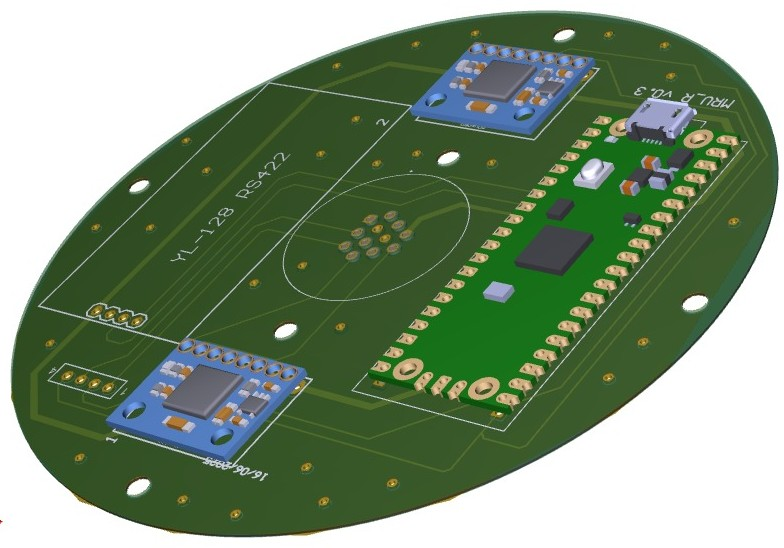
\includegraphics[height=5.5cm]{imagens/3d_prot1a.jpeg}
        }\hfill
        \subfloat[PCB Lado Traseiro]{
            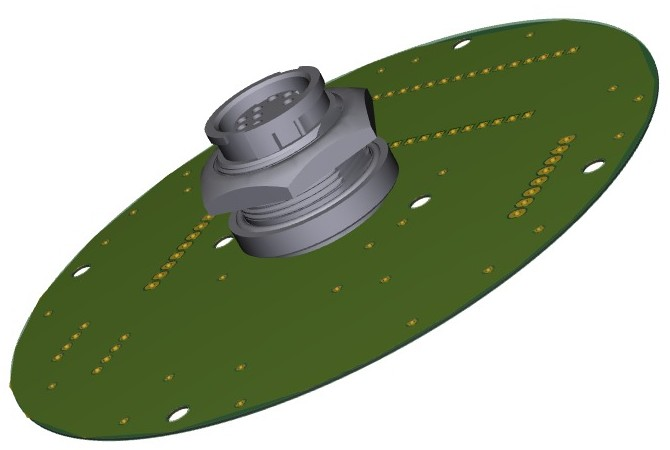
\includegraphics[height=5.5cm]{imagens/3d_prot1b.jpeg}
        }

        \textbf{Fonte}: Autoria Própria
        \label{fig:pcb1}
    \end{figure}

    \vspace{1cm}

    \begin{figure}[H]
        \centering
        \caption{PCB 3D do Protótipo 02}
        
        \subfloat[PCB Lado Frontal]{
            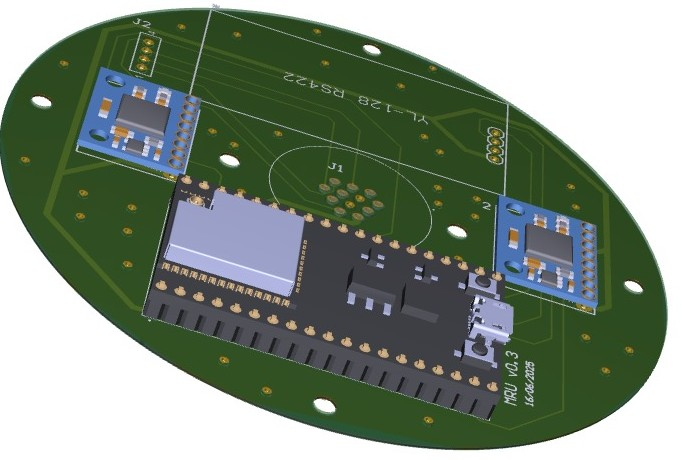
\includegraphics[height=5.5cm]{imagens/3d_prot2a.jpeg}
        }
        \subfloat[PCB Lado Traseiro]{
            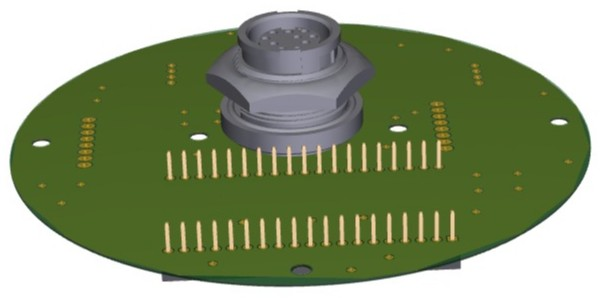
\includegraphics[height=4.5cm]{imagens/3d_prot2b.jpeg}
        }

        \textbf{Fonte}: Autoria Própria
        \label{fig:pcb1}
    \end{figure}



\newpage
\setcounter{section}{5}
\section{Design da Embalagem}
    A embalagem do projeto foi elaborada em formato cilíndrico, formato similar a outros dispositivos DDRM similares no mercado com intuito de garantir a estabilidade do sistema. No primeiro desenho (Figura\autoref{fig:embfinal}), observa-se a parte superior da embalagem do DRMM, composta por uma tampa metálica parafusada, que assegura a vedação do sistema contra agentes externos como umidade, salinidade e poeira, em conformidade com os requisitos de robustez para aplicações offshore. A presença de prensa-cabos reforça a proteção dos pontos de entrada de fios e cabos, viabilizando a conexão elétrica e de dados sem comprometer a estanqueidade do invólucro. 

    \begin{figure}[H]
        \centering
        \caption{Ilustração 3D Protótipo}
        
        \subfloat[Desenhos]{
            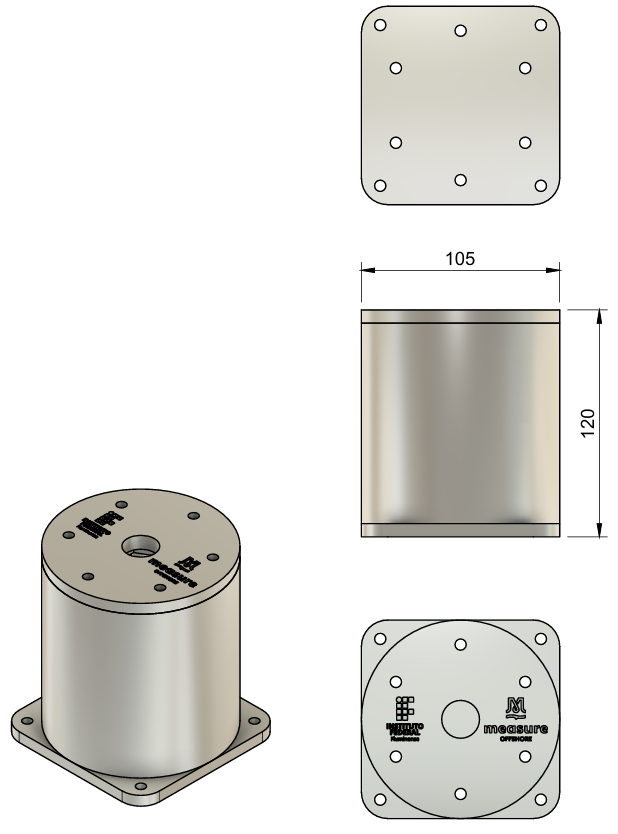
\includegraphics[height=9.5cm]{imagens/desenho1.PNG}
        }\hfill
        \subfloat[Ilustração]{
            \frame{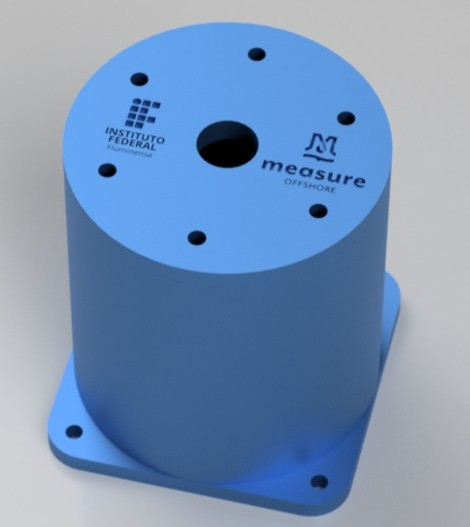
\includegraphics[height=9.5cm]{imagens/emb3d2.jpeg}}
        }

        \textbf{Fonte}: Autoria Própria
        \label{fig:embfinal}
    \end{figure}

    A embalagem consiste em um invólucro cilíndrico de 105 mm de diâmetro por 120 mm de altura, apoiado sobre uma base quadrada de 105 $\times$ 105 mm com quatro flanges e furos M5 para fixação. A tampa superior tem um furo central para passagem de cabos e oito furos periféricos para parafusos, garantindo fechamento estanque. Ademais, o compartimento será usinado em alumínio anodizado e pintado em azul náutico para resistência à corrosão e dissipação térmica, inclui gaxetas de silicone para vedação IP67, logos institucionais gravados e design modular que facilita manutenção e assegura estabilidade e proteção da eletrônica do DRMM em ambientes offshore. As figuras subsequentes mostram as outras partes do sistema em seus respectivos desenhos técnicos e esquematizações 3D.


    \begin{figure}[H]
        \centering
        \caption{Desenhos Técnicos e Esquematizações 3D da Embalagem}

        \subfloat[Corpo da Embalagem]{
            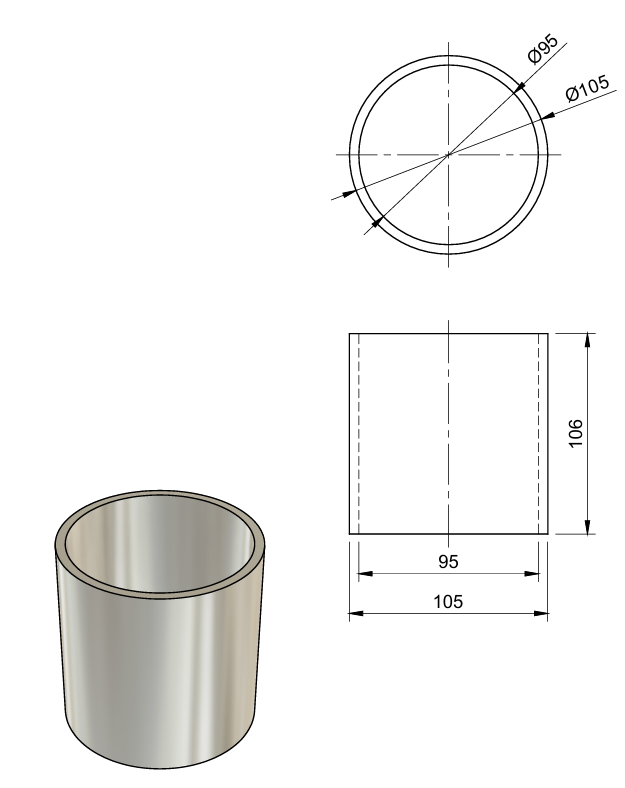
\includegraphics[height=10.2cm]{imagens/desenho2.PNG}
        }\hfill
        \subfloat[Base da Embalagem]{
            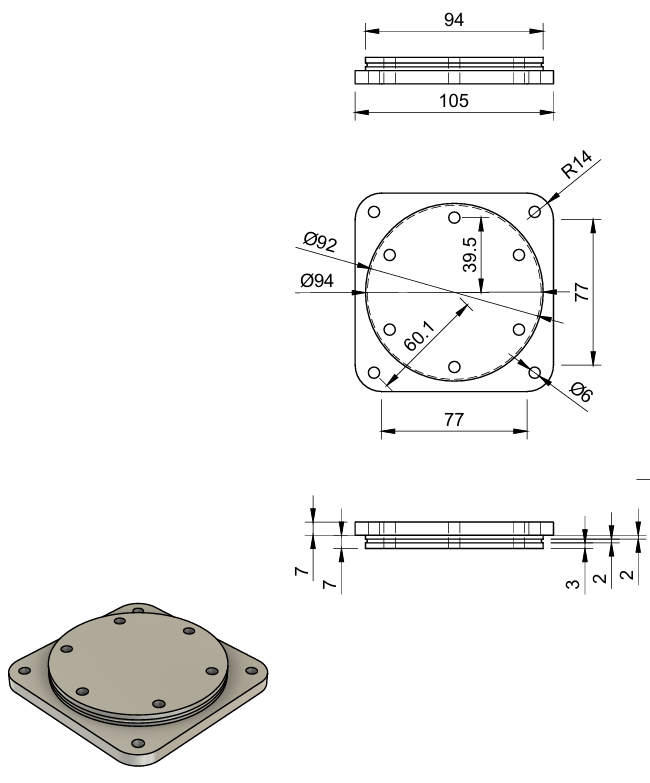
\includegraphics[height=10.1cm]{imagens/desenho3.PNG}
        }
        
        \subfloat[Tampa da Embalagem]{
            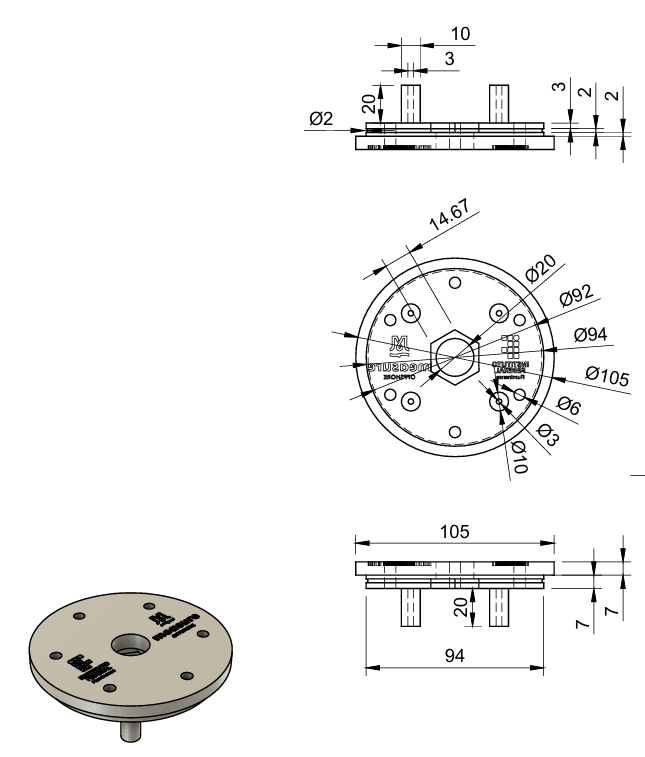
\includegraphics[height=10.1cm]{imagens/desenho4.PNG}
        }
        
        \label{fig:enter-label}
        \textbf{Fonte:} Autoria Própria
    \end{figure}


\newpage
\section{Considerações Finais}
\addcontentsline{toc}{section}{Considerações Finais}
    Dado o exposto, diversos aprimoramentos e esquematizações foram realizados com o objetivo de preparar o terreno para a fase de testes e prototipagem do dispositivo. Nesse sentido, não apenas a estrutura geral do sistema que integrará o DRMM foi definida, como também foram desenvolvidos o projeto da placa de circuito impresso e o desenho técnico da embalagem. Esses avanços representam um marco importante na consolidação de um dispositivo confiável, robusto e adequado às exigências do ambiente offshore, evidenciando o progresso técnico alcançado na construção de uma solução nacional compatível com os padrões internacionais de desempenho e segurança.
    
    Como conteúdo complementar, também foram apresentados os estudos que fundamentam as técnicas de filtragem aplicadas aos sensores, com o intuito de minimizar o ruído e extrair de forma mais precisa os sinais relevantes de cada variável monitorada. Além disso, foram exploradas abordagens avançadas de fusão de dados, como os algoritmos de Kalman e Covariance Intersection, que permitem combinar informações de múltiplos sensores para gerar estimativas mais robustas. Complementarmente, abre-se espaço para a aplicação de algoritmos de aprendizado de máquina, capazes de “aprender” com sensores de alta precisão e, assim, elevar o desempenho do sistema para níveis superiores aos limitados pelo hardware e componentes básicos utilizados, representando um avanço significativo em termos de inteligência embarcada e adaptabilidade do dispositivo.

    Dessa forma, conclui-se que o projeto alcançou um grau significativo de maturidade, encontrando-se apto para a realização de testes em laboratório e para a construção do sistema completo. Os próximos passos envolvem a otimização das soluções já desenvolvidas, com foco na avaliação de sensores e microprocessadores mais precisos e com melhor relação custo-benefício, além do aprimoramento dos algoritmos implementados, visando aumentar a eficiência do processamento e garantir tempos de amostragem compatíveis com as exigências do mercado. Paralelamente, o design da embalagem também poderá ser refinado, considerando aspectos térmicos, como o aquecimento dos componentes internos e a necessidade de uma dissipação de calor mais eficiente, assegurando a estabilidade operacional do sistema em ambientes offshore.


\newpage
\newpage

% ATIVA O CABEÇALHO DAS REFERÊNCIAS
\pagestyle{modeloReferencias}

% ADICIONA UM TIPO "SECTION" CUSTOMIZADO NO SUMÁRIO
\addcontentsline{toc}{section}{Referências}

% CRIA UMA SECTION SEM NUMERAÇÃO
\section*{Referências}
\vspace{-1cm}

%\hyperlink{MARINHA}{(MARINHA, 2017)}



\referencia
    {DINGLER}
    {Arvid et al. Aplicação do Filtro de Kalman Unscented para Estimativa do Fluxo. Projeto de pesquisa, UFF}
    {2024}
    {\url{https://www.mathworks.com/help/matlab/ref/quiver3.html}}
    {26 jun. 2025}

\referencia
    {EIBENSTEIN}
    {Arvid et al. A study on band‑pass filtering for calculating foot displacements from accelerometer and gyroscope sensors}
    {2009}
    {\url{https://pubmed.ncbi.nlm.nih.gov/19963857/}}
    {10 mai. 2025}

\referencia
    {MATHWORKS}
    {Inc. quiver3 – 3-D quiver or vector plot. MathWorks Documentation}
    {2025}
    {\url{https://dev.to/sebastian_dingler/a-gentle-introduction-to-covariance-intersection-1bpa}}
    {19 jun. 2025}

\referencia
    {NATIONAL INSTRUMENTS}
    {Integration – Sound and Vibration Toolkit User Manual. LabVIEW}
    {2024}
    {\url{https://www.ni.com/docs/en-US/bundle/labview-sound-and-vibration-toolkit/page/integration.html}}
    {12 jun. 2025}

\referencia
    {NPX}
    {Implementing a Tilt‑Compensated eCompass using Accelerometer and Magnetometer Sensors, Application Note AN4248, NXP / Freescale Semiconductor}
    {2010}
    {\url{https://www.nxp.com/docs/en/application-note/AN4248.pdf}}
    {22 mai. 2025}

\referencia
    {SCIELO}
    {Sutileza dos Quatérnions no Movimento de Rotação de Corpos. Revista Brasileira de Educação Física e Esporte}
    {2020}
    {\url{https://www.scielo.br/j/rbef/a/XvBQPp9F5SsWwQCTGX9pk5C/?utm_source=chatgpt.com}}
    {22 mai. 2025}

\referencia
    {STANFORD}
    {EE267: IMU Notes. Stanford University}
    {2019}
    {\url{https://stanford.edu/class/ee267/notes/ee267_notes_imu.pdf}}
    {26 mai. 2025}

\referencia
    {TAWIL}
    {Yahya. Towards understanding IMU: Basics of Accelerometer and Gyroscope Sensors and How to Compute Pitch, Roll and Yaw Angles. Atadiat}
    {2023}
    {\url{https://atadiat.com/en/e-towards-understanding-imu-basics-of-accelerometer-and-gyroscope-sensors/}}
    {12 jun. 2025}

\referencia
    {UFF}
    {Arvid et al. Aplicação do Filtro de Kalman Unscented para Estimativa do Fluxo. Projeto de pesquisa, UFF}
    {2009}
    {\url{https://app.uff.br/riuff/bitstream/handle/1/29420/Project.pdf}}
    {14 mai. 2025}

\referencia
    {WRIGHT}
    {Stephanie Burrell. Understanding the Cutoff Frequency for a Low Pass Filter: A Beginner's Guide}
    {2024}
    {\url{https://wraycastle.com/blogs/knowledge-base/cutoff-frequency-for-a-low-pass-filter}}
    {10 mai. 2025}


\phantom{a}

\newpage
    \thispagestyle{empty}
    \centering
    \phantom{a}
    \vfill

    \addcontentsline{toc}{section}{Anexos}
    \Large
    \textbf{Anexos}
    
    \vfill
    \phantom{a}
\newpage

\begin{figure}[H]
    \centering
    \caption{Folha 1 Desenho V2}
    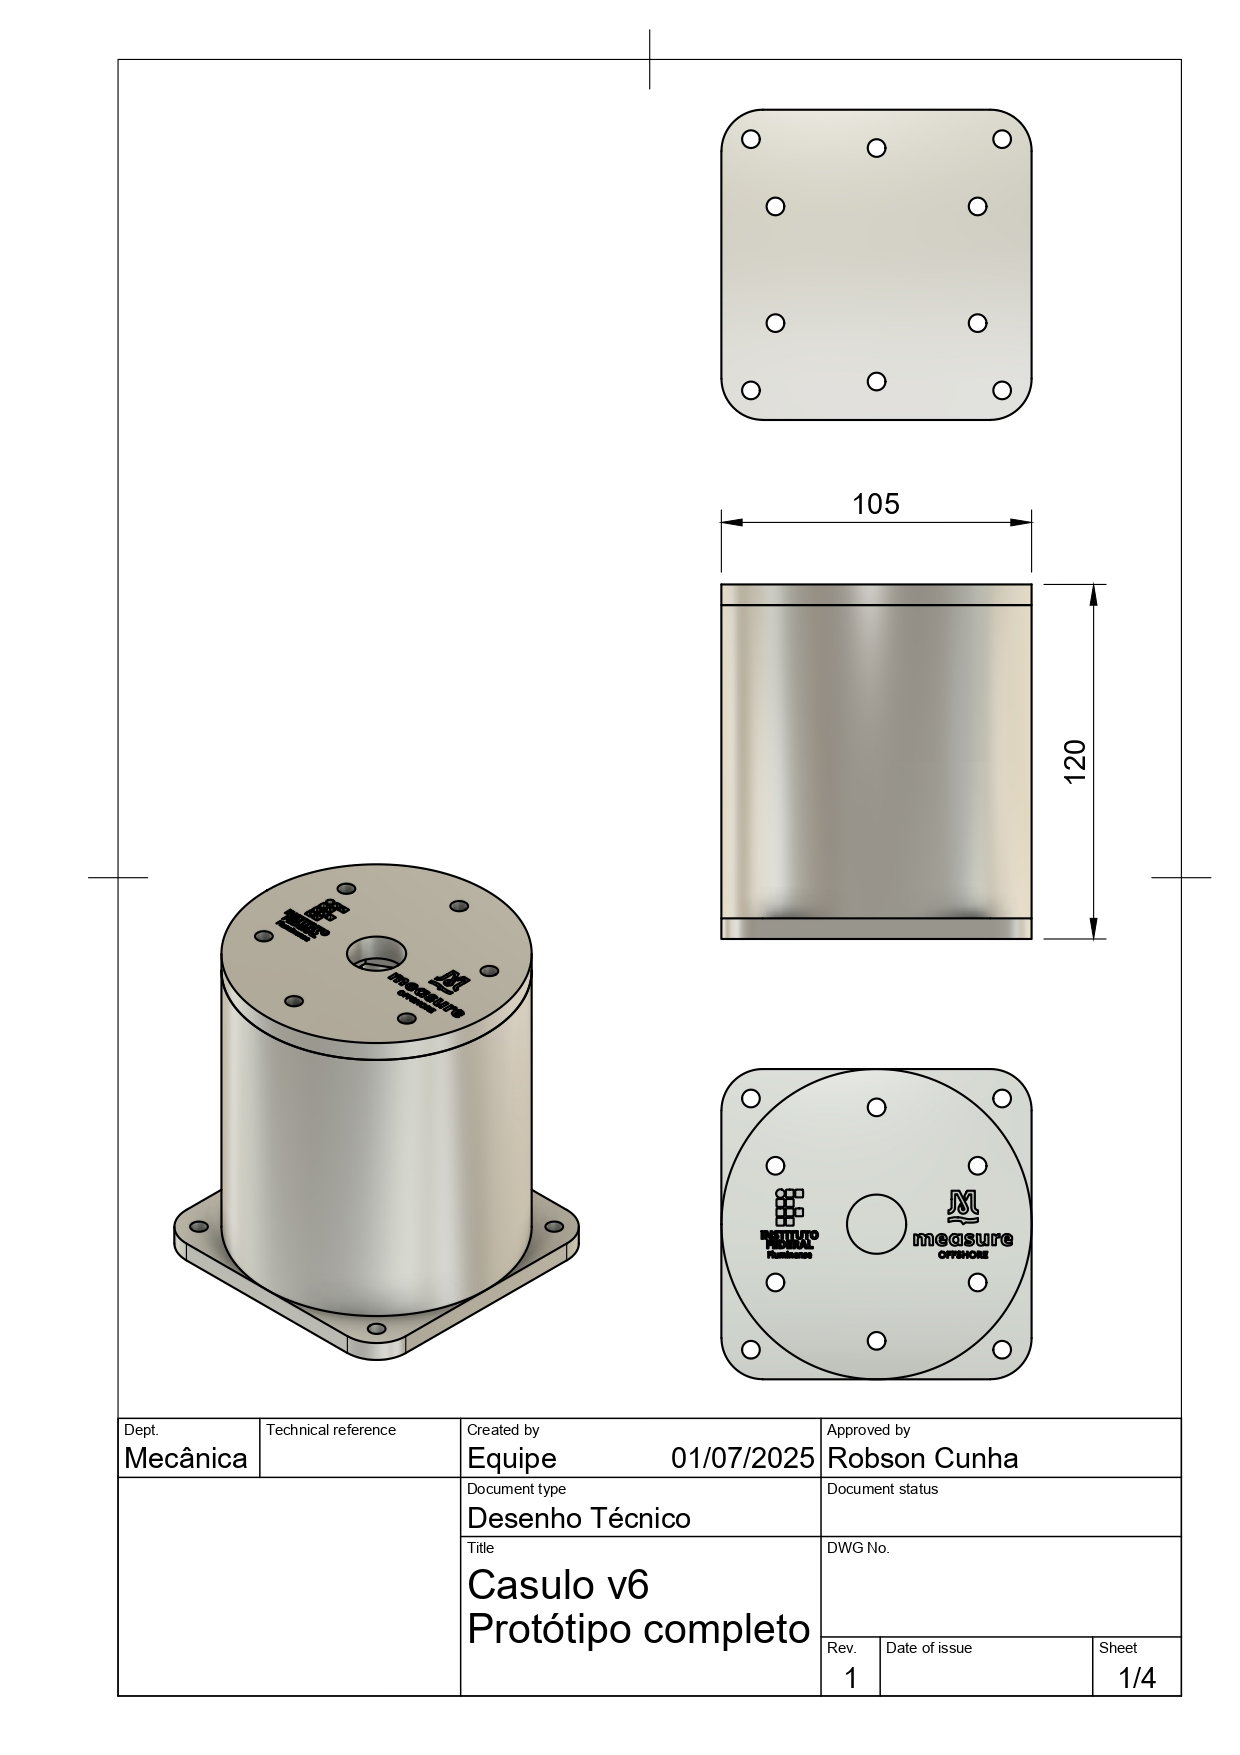
\includegraphics[width=.95\linewidth]{imagens/Folha 1 Desenho v2_page-0001.jpg}
    
    \label{fig:enter-label}
    \textbf{Fonte: } Autoria Própria
\end{figure}

\newpage

\begin{figure}[H]
    \centering
    \caption{Folha 2 Desenho V2}
    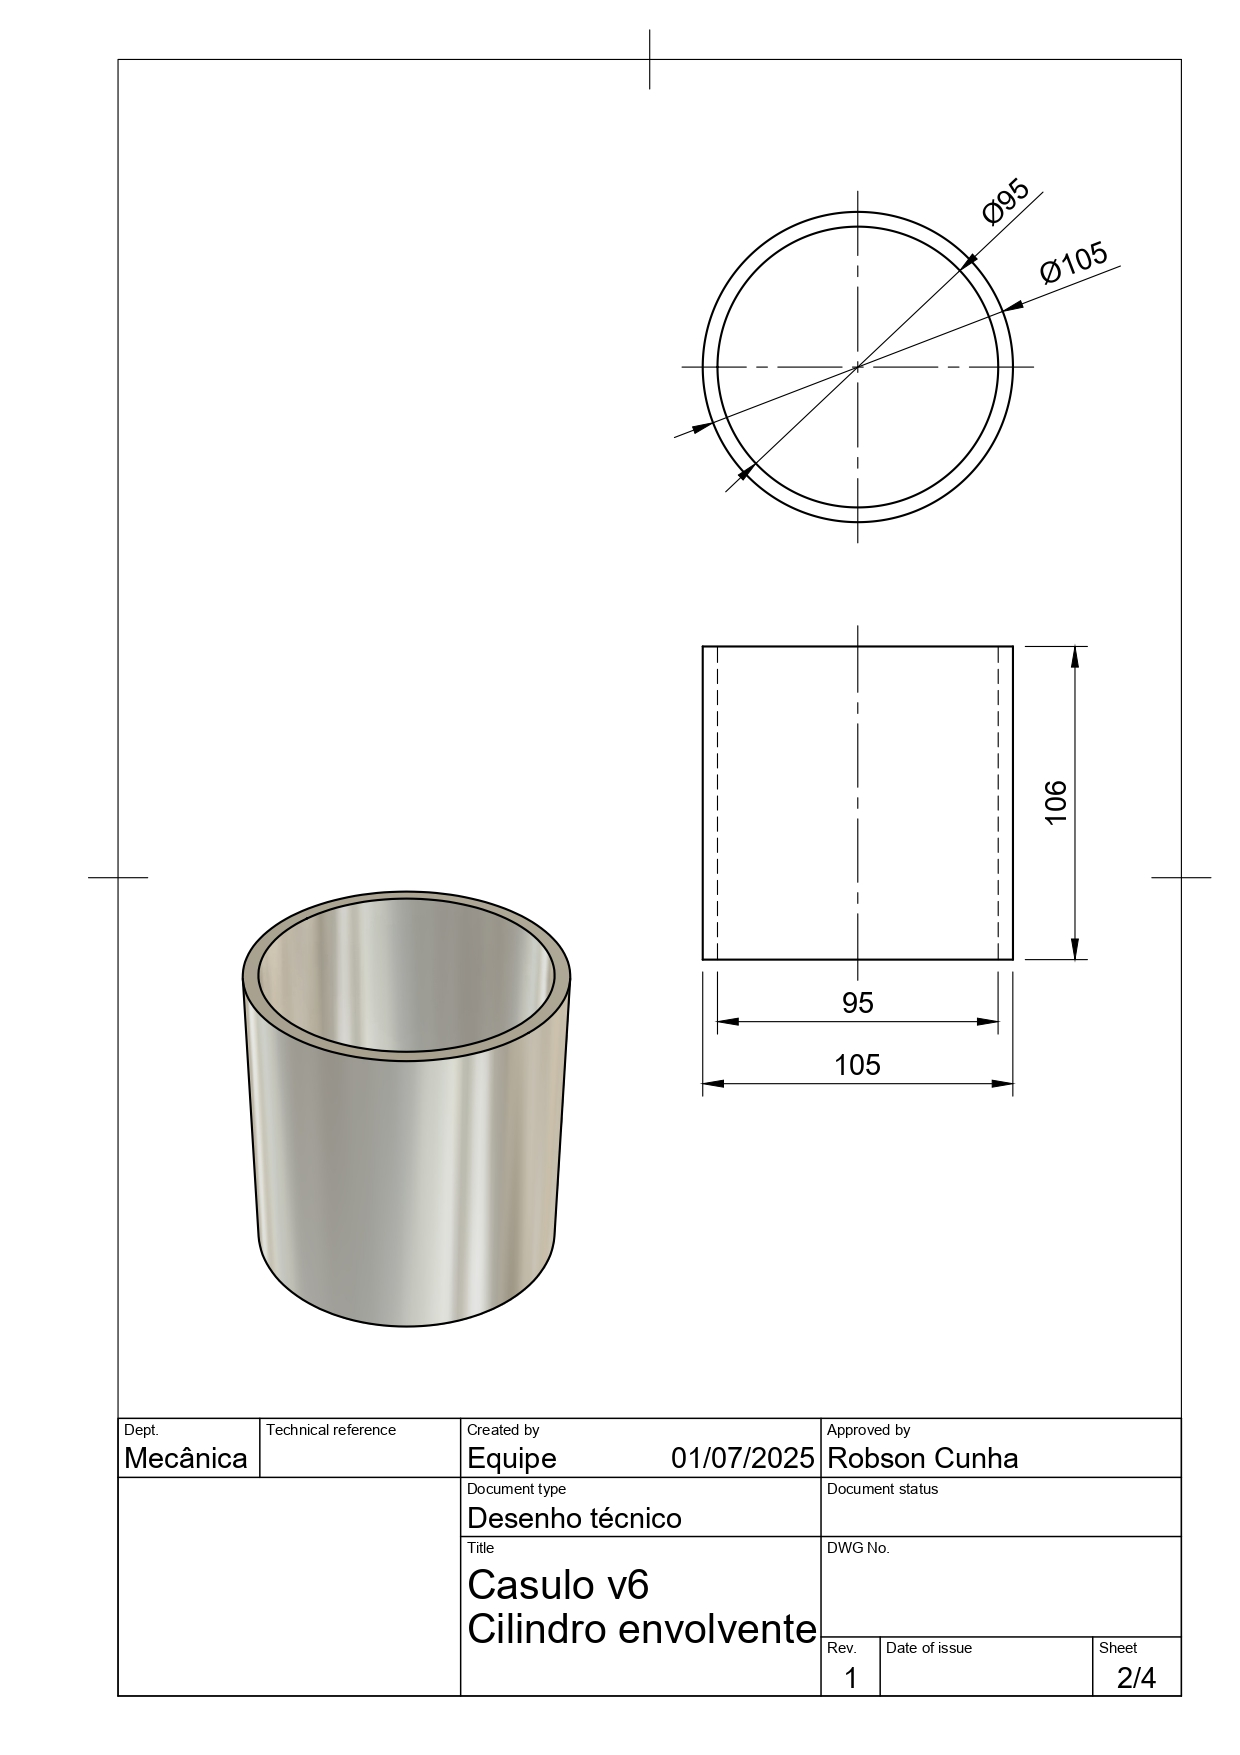
\includegraphics[width=.95\linewidth]{imagens/Folha 2 Desenho v2_page-0001.jpg}
    
    \label{fig:enter-label}
    \textbf{Fonte: } Autoria Própria
\end{figure}

\newpage

\begin{figure}[H]
    \centering
    \caption{Folha 3 Desenho V2}
    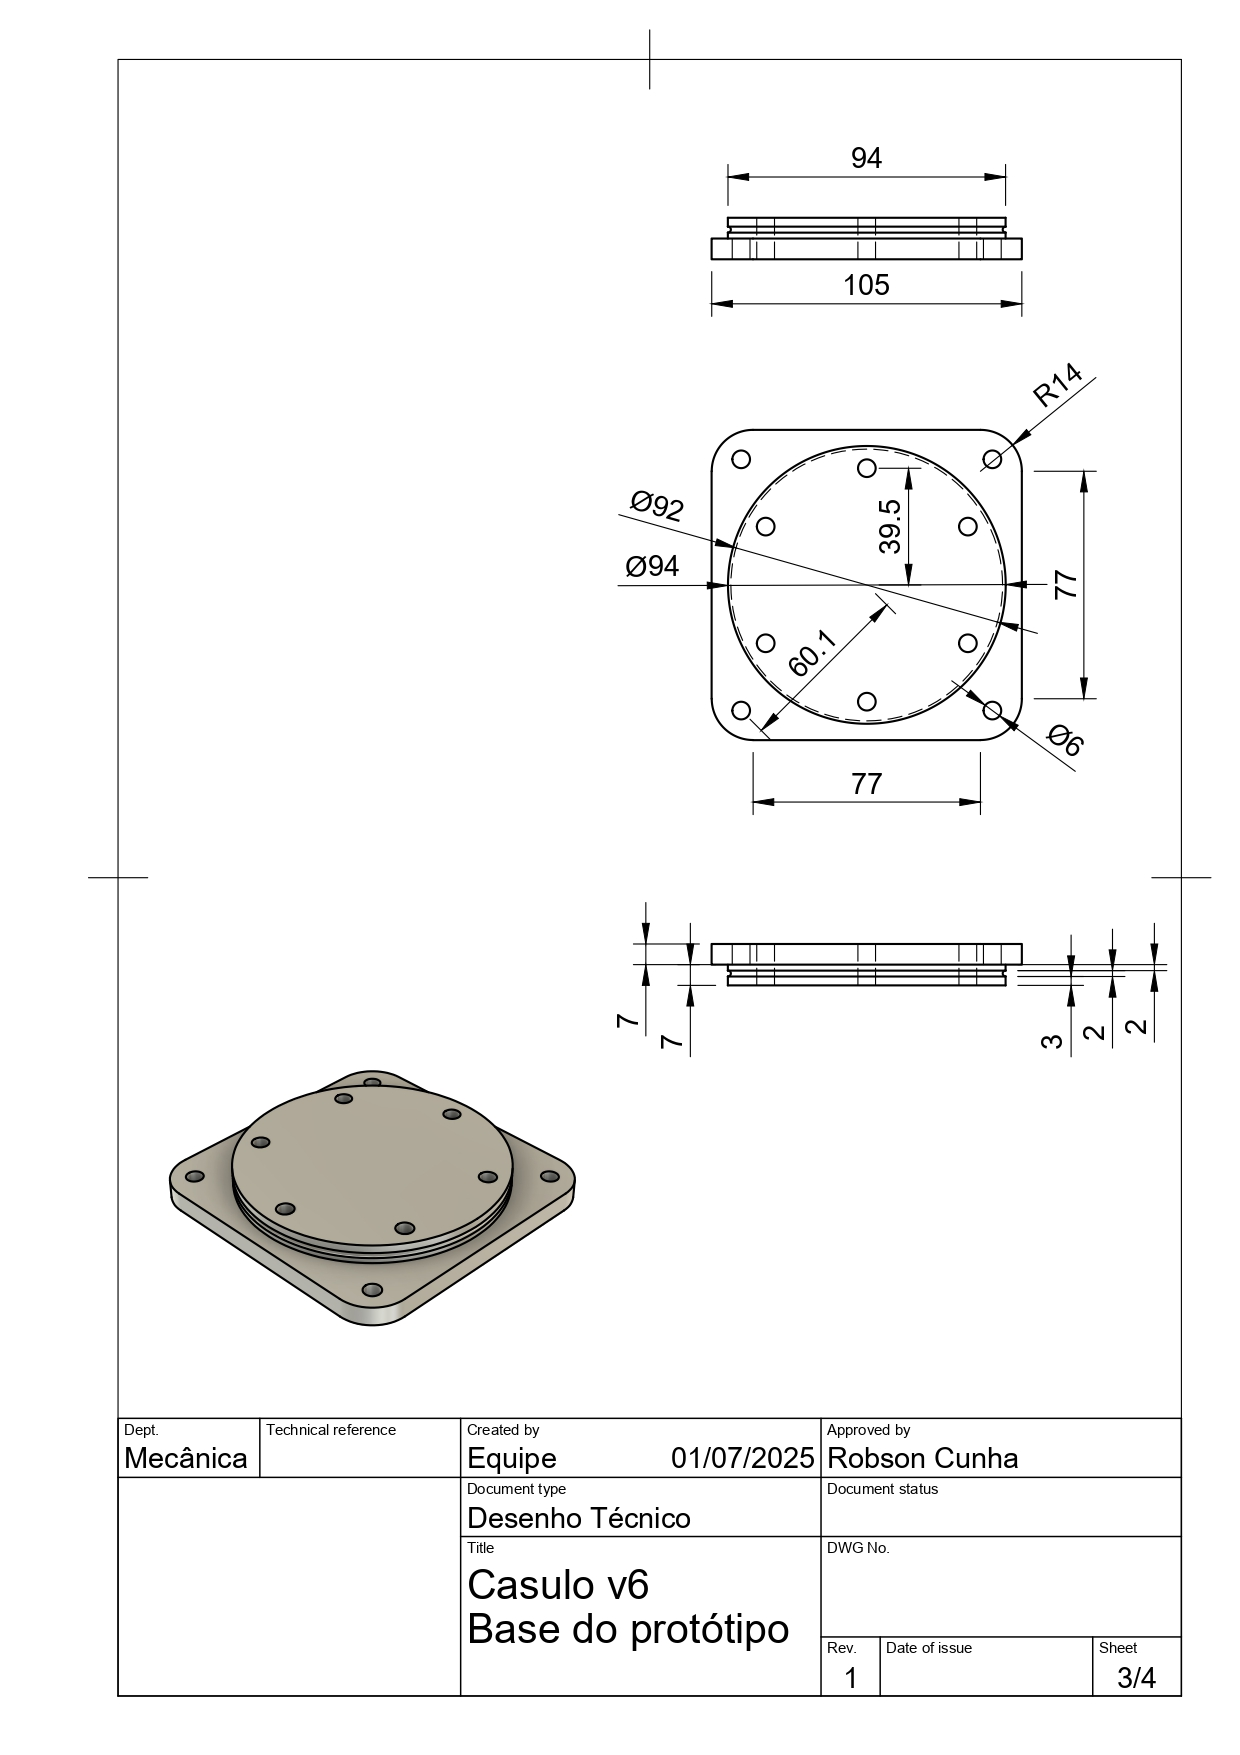
\includegraphics[width=.95\linewidth]{imagens/Folha 3 Desenho v2_page-0001.jpg}
    
    \label{fig:enter-label}
    \textbf{Fonte: } Autoria Própria
\end{figure}

\newpage

\begin{figure}[H]
    \centering
    \caption{Folha 4 Desenho V2}
    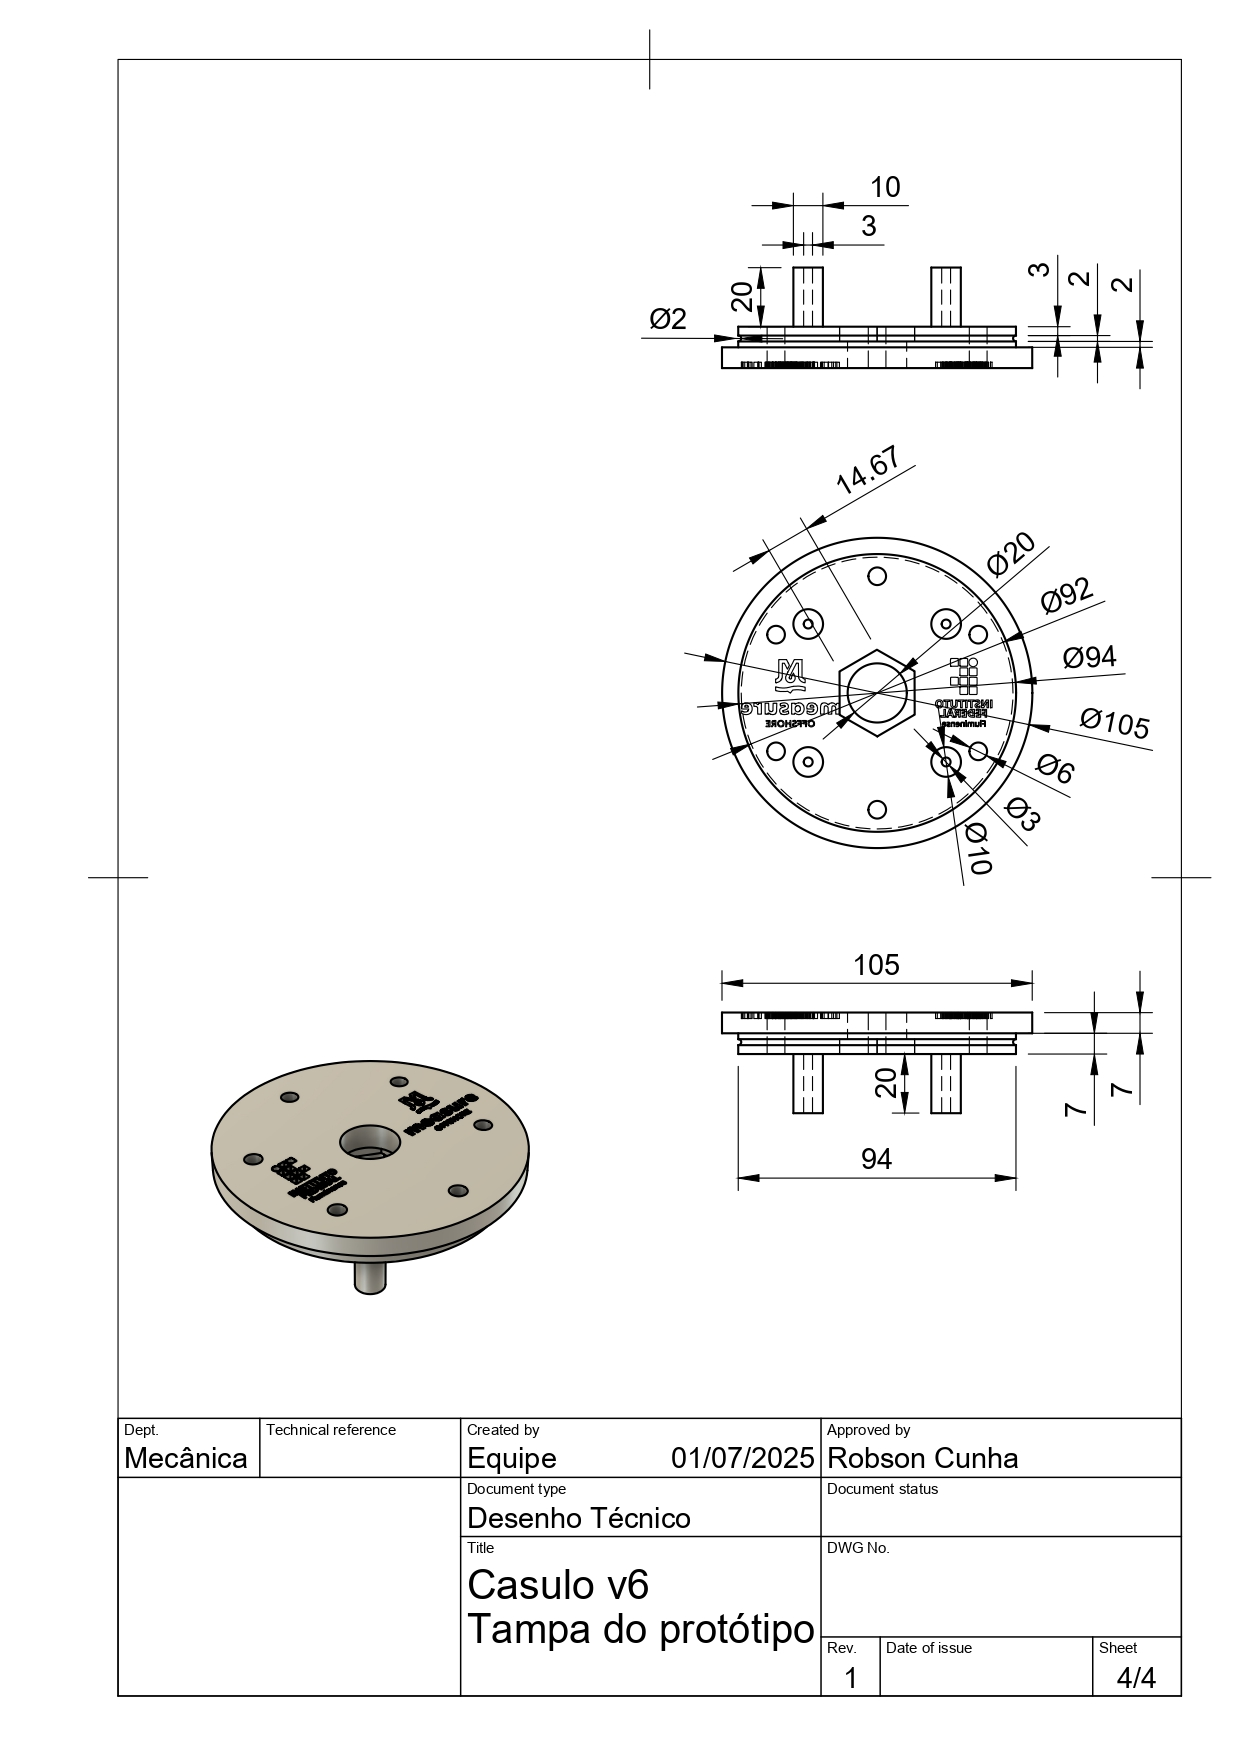
\includegraphics[width=.95\linewidth]{imagens/Folha 4 Desenho v2_page-0001.jpg}
    
    \label{fig:enter-label}
    \textbf{Fonte: } Autoria Própria
\end{figure}

\newpage
\end{document}